%%
%% $Id$
%%
%% Copyright (c) 2007-2008 Christian Fehler
%% Copyright (c) 2007-2008 Benjamin Mies
%%


\documentclass[twoside]{report}


\usepackage[utf8]{inputenc}
\usepackage[ngerman]{babel}
\usepackage{textcomp}
\usepackage{longtable}
\usepackage{amsmath}
\usepackage{amssymb}
\usepackage{amstext}
\usepackage{latexsym}
\usepackage{array}
\usepackage{stmaryrd}
\usepackage[a4paper,
            colorlinks=false,
            final,
            pdfkeywords={Lernwerkzeug fuer die Grundlagen der theoretischen Informatik},
            pdftitle={Lernwerkzeug fuer die Grundlagen der theoretischen Informatik},
            pdfauthor={Christian Fehler, Benjamin Mies},
            pdfsubject={Diplomarbeit},
            pdfdisplaydoctitle=true]{hyperref}
\usepackage{graphicx}
\usepackage{cite}


\pagestyle{headings}


%%
%% $Id$
%%
%% Copyright (c) 2007-2008 Christian Fehler
%% Copyright (c) 2007-2008 Benjamin Mies
%%


\usepackage{color}

\newcommand{\gtitool}[0]{GTI Tool\ }
\newcommand{\gtitools}[0]{GTI Tools\ }


\newcommand{\gticite}[1]{\cite{#1}}
\newcommand{\gticitepage}[2]{\cite[S. #2]{#1}}


\definecolor{ColorState}{rgb}{0.0,0.0,0.5}
\definecolor{ColorSymbol}{rgb}{0.0,0.0,0.5}
\definecolor{ColorNonterminalSymbol}{rgb}{0.0,0.5,1.0}
\definecolor{ColorStartSymbol}{rgb}{0.5,0.0,1.0}
\definecolor{ColorTerminalSymbol}{rgb}{0.0,0.0,0.5}


\newcommand{\State}[1]{\textbf{\color{ColorState}#1}}

\newcommand{\Word}[1]{\textbf{\color{ColorSymbol}#1}}

\newcommand{\Symbol}[1]{\textbf{\color{ColorSymbol}#1}}
\newcommand{\Symbols}[1]{\textbf{\color{ColorSymbol}\texttt{\dq}#1\texttt{\dq}}}
\newcommand{\SymbolEmpty}[0]{\textbf{\color{ColorSymbol}\texttt{\dq}}}

\newcommand{\NonterminalSymbol}[1]{\textbf{\color{ColorNonterminalSymbol}#1}}
\newcommand{\NonterminalSymbols}[1]{\textbf{\color{ColorNonterminalSymbol}\texttt{\dq}#1\texttt{\dq}}}

\newcommand{\StartSymbol}[1]{\textbf{\color{ColorStartSymbol}#1}}
\newcommand{\StartSymbols}[1]{\textbf{\color{ColorStartSymbol}\texttt{\dq}#1\texttt{\dq}}}

\newcommand{\TerminalSymbol}[1]{\textbf{\color{ColorTerminalSymbol}#1}}
\newcommand{\TerminalSymbols}[1]{\textbf{\color{ColorTerminalSymbol}\texttt{\dq}#1\texttt{\dq}}}


\title{
{\huge Diplomarbeit}\\[10mm]
{\Huge Lernwerkzeug für die Grundlagen der theoretischen Informatik}}

\author{
{\Large Christian Fehler}\\[1mm]
Matr.Nr. 664828\\[4mm]
{\Large Benjamin Mies}\\[1mm]
Matr.Nr. 662891\\[6mm]
Fachbereich 12 - Informatik und Elektrotechnik\\[1mm]
Fachgruppe Programmiersprachen\\[1mm]
Universität Siegen\\[6mm]
\begin{tabular}{rl}
Gutachter: & Privatdozent Dr. Kurt Sieber\\
           & Dipl.-Inform. Benedikt Meurer
\end{tabular}
}

\date{\small Abgabedatum: \ClosingDate}

\setcounter{secnumdepth}{3}


\begin{document}

\maketitle

\tableofcontents
\newpage

\setcounter{secnumdepth}{-1}
%%
%% $Id$
%%
%% Copyright (c) 2007-2008 Christian Fehler
%% Copyright (c) 2007-2008 Benjamin Mies
%%


\chapter{Einleitung}\label{Introduction}

Das Fach Grundlagen der theoretischen Informatik ist für alle
Informatikstudenten der Universität Siegen eine Pflichtveranstaltung. Allerdings
haben bisherige Klausurergebnisse gezeigt, dass einige Studenten Probleme mit
diesem Themengebiet haben.\vspace{10pt}

Um die Studenten bei der Lösung dieser Probleme zu unterstützen, ist die Idee
entstanden, ein Lernwerkzeug für dieses Fach zu entwickeln. Dieses Lernwerkzeug
soll den Stoff der Vorlesung und der Übungen abdecken, und den Studenten helfen,
diesen besser nachvollziehen zu können, um Verständnisprobleme zu
beseitigen.\vspace{10pt}

Dieses Lernwerkzeug haben wir im Rahmen unserer Diplomarbeit entwickelt, und im
Folgenden soll vorgestellt werden, welche Funktionen bereits verfügbar sind. In
Kapitel \ref{Perspective} werden wir noch auf zukünftige Aussichten für dieses
Projekt eingehen, wobei wir Erweiterungsmöglichkeiten nennen und einen Vorschlag
für die Realisierung geben werden.\vspace{10pt}

\setcounter{secnumdepth}{2}

%%
%% $Id$
%%
%% Copyright (c) 2007-2008 Christian Fehler
%% Copyright (c) 2007-2008 Benjamin Mies
%%


\chapter{Oberfläche}\label{GUI}

In diesem Kapitel geht es um die Oberflächengestaltung. Zum einen geht es darum,
wie und warum die Hauptansicht so gestaltet wurde, zum anderen darum, welche
besonderen Schritte notwendig waren, um das Aussehen zu verbessern und dem
Benutzer es dadurch zu erleichtern mit dem \gtitool zu arbeiten.


\section{Gestaltung der Hauptansicht}

Als wir zu Beginn der Diplomarbeit über die Gestaltung der Hauptansicht
diskutiert haben, kamen wir sehr schnell zu der Übereinkunft, dass die
Ähnlichkeit zu dem Lernwerkzeug TPML möglichst hoch sein sollte. Da sowohl die
Veranstaltung "`Grundlagen der theoretischen Informatik"', als auch "`Theorie
der Programmierung I"' für jeden Informatikstudenten der Universität Siegen
Pflichtveranstaltungen sind, ist die Wahrscheinlichkeit, dass Studenten beide
Lernwerkzeuge nutzen werden sehr hoch.\vspace{10pt}

Ein großer Vorteil von dieser Entscheidung war natürlich, dass wir beide
bereits an der Projektgruppe TPML mitgearbeietet hatten. Zwar waren wir nicht
hauptsächlich für die Grafikelementen beteiligt, konnten aber dennoch einige
Einblicke sammeln, welche uns bei der Grafikgestaltung sehr geholfen
haben.\vspace{10pt}

Unserer Hoffnung ist es, dass zukünftige Benutzer von den parallelen im Aussehen
und in der Funktionsweise beider Lernwerkzeuge profitieren können.\vspace{10pt}

Während der gesamten Diplomarbeit stand im Vordergrund das Lernwerkzeug so
intuitiv und selbsterklärend wie möglich zu gestalten. Denn schließlich soll
ein Benutzer nicht noch lange zeit darauf verwenden müssen, den Umgang mit dem
Werkzeug zu erlernen und sich im schlimmsten Falle durch ein dickes Handbuch
durchzuarbeiten.\vspace{10pt}

Aus diesem Ansatz heraus ist zum Beispiel auch der Wizard zum Anlegen einer
neuen Datei enstanden. Dieser Wizard hat für jedes Eingabefeld ja schon einen
Vorschlag, welche in den Einstellungen auf die Benutzerwünsche angepasst werden
kann. Beim ersten Start sollen diese Werte allerdings als Orientierung und
Beispieldaten dienen, was an diesen Stellen eingetragen werden soll.


\section{Redo/Undo}

Da das Lernwerkzeug vom Aussehen her sehr an einen Editor angelehnt ist,
wollten wir dem Benutzer auch eine Möglichkeit geben Schritte rückgängig zu
machen oder wiederherzustellen. Dies war jedoch zu einem Zeitpunkt, zu dem bei
weitem noch nicht alle Funktionalität implementiert war. Desweiteren soll das
Werkzeug ja auch zukünftig an den Stoff der Vorlesung angepasst werden, so dass
uns eine einfache Erweiterbarkeit sehr wichtig war.\vspace{10pt}

Daher haben wir uns entschlossen die Verwaltung der Redo/Undo Schritte nicht
einer Klasse alleine zu überlassen, sondern die verschiedenen Aktionen in
einzelnen Items zu kapseln. Auf diesen Items kann dann die entsprechende redo
bzw. undo Funktion aufgerufen werden. Verwaltet wird dies von einem Handler,
welcher sich nur merkt welches das letzte aktive Item für Redo und Undo ist,
und den Aufruf durch den Nutzer an das Item weiterleitet.\vspace{10pt}

Durch diese Kapselung ist es leicht möglich die Redo/Undo Funktion zu
erweitern, da einfach ein neues Item für die entsprechende Aktion implementiert
werden muss, um diese Item beim Ausführen der Aktion an den Handler zu
übergeben.


\section{Anpassung aller GUI Komponenten}

Ein wichtiges Konzept bei der graphischen Gestaltung des \gtitool ist es, die von
der Programmiersprache zur Verfügung gestellten Komponenten anzupassen und dann
nur noch ausschließlich diese angepassten Komponenten zu benutzen. Der wohl
größte Vorteil dieser Umsetzung ist, dass nicht überall ein normaler String
verwendet wird, sondern ein sogenannter PrettyString. Dieser enthält neben dem
normalen Text auch noch Farbinformation, sowie Zeichenattribute, wie zum
Beispiel Fettdruck.\vspace{10pt}

Der erforderliche Aufwand wurde investiert, um dem Benutzer eine möglichst
ansprechende Oberfläche zu präsentieren und ihn durch die zusätzlichen
Informationen zu unterstützen, die Inhalte besser zu verstehen.\vspace{10pt}

Ein weiterer wichtiger Ansatz war, dass der Benutzer das \gtitool möglichst
intuitiv bedienen kann. Um dies umzusetzen, wurde unter anderen Drag and Drop
auf den verschiedenen Komponenten implementiert. So kann der Benutzer im
Übergangs-Dialog die Symbole einfach vom "`Alphabet"' in die
"`Übergangs-Menge"' ziehen. Gleiches gilt für das Umsortieren von Produktionen,
das zwar die Grammatik nicht ändert, aber es dem Benutzer ermöglicht die
Produktionen übersichtlicher anzuordnen. In vielen Programmen, in denen Tabs
zur Gliederung benutzt werden, gehört es zum Funktionsumfang diese Tabs per Drag
and Drop zu verschieben. Auch dies wurde implementiert, da es dem Benutzer
erlaubt, seine Daten besser zu organisieren.


\section{Look \& Feel}\label{LookAndFeel}

Damit das \gtitool unter verschiedenen Betriebsystemen immer gleich, oder
zumindest sehr ähnlich aussieht, kam während der Entwicklung der Wunsch auf, ein
eigenes Look \& Feel zu verwenden. Java bietet in diesem Bereich zwar mit dem
Metal Look \& Feel eine Lösung an, die unter allen Betriebsystemen gleich
aussehen soll, diese erfüllte aber unsere Vorstellungen nicht. Schließlich fiel
die Wahl auf TinyLaF, ein weitestgehend gezeichnetes Look \& Feel, dass somit
unter allen Betriebsystemen gleich aussieht. Dem Benutzer ist es aber
freigestellt ein anderes, zum Beispiel das normale Betriebsystem Look \& Feel zu
verwenden, wenn er dies wünscht. Alle in dieser Arbeit verwendeten Bilder des
\gtitools wurden mit TinyLaF als Look \& Feel gemacht.


\section{Zweite Ansicht}\label{SecondView}

Bei der Umsetzung der verschiedenen Algorithmen wurden wir vor das Problem
gestellt, dass es sinnvoll wäre, einen Automaten nach der Umwandlung, mit dem
Automaten oder der Grammatik vor der Umwandlung zu vergleichen. Dies war nur
durch einen Tabwechsel oder das Öffnen eines zweiten \gtitools möglich, was
nicht besonders benutzerfreundlich war.\vspace{10pt}

\begin{figure}[h!]
\begin{center}
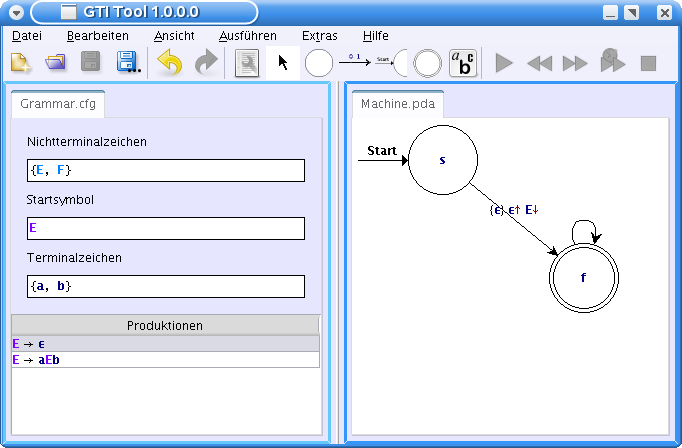
\includegraphics[width=12cm]{../images/second_view.png}
\caption{Zweite Ansicht}
\end{center}
\end{figure}

Das Problem wurde dadurch gelöst, dass eine zweite Ansicht integriert wurde,
die es erlaubt, Tabs in einem zweiten Bereich zu öffnen, so dass zwei Dateien
gleichzeitig sichtbar sind. Während der Umsetzung mussten verschiedene Probleme
diskutiert und gelöst werden. So stellte sich die Frage, wie dem Benutzer
verdeutlicht werden kann, welche der beiden sichtbaren Dateien aktiv ist.
Wichtig ist dieser Status für die Aktivierung der Menüeinträge bzw. Toolbar
Buttons. Als Umsetzung wurde schließlich ausgewählt, dass anhand von
unterschiedlichen Umrandungen dem Benutzer klar gemacht werden soll, welche der
beiden Dateien die aktive ist. Durch dieses Vorgehen wird intuitiv klar, welche
Datei aktiv ist, da sich die Farbe der Umrandung beim Aktivieren der anderen
Ansicht ändert.\vspace{10pt}

Eine weitere wichtige Eigenschaft der zweiten Ansicht ist es, dass Dateien in
diese zweite Ansicht verschoben werden können müssen. Ebenfalls muss es möglich
sein in der zweiten Ansicht Dateien zu öffnen, bzw. neue zu erstellen. Um die
letzen beiden genannten Punkte umzusetzen, wurde das Konzept des aktiven
Editors erweitert. Die oben beschriebene andere Darstellung der aktiven Datei
wurde so erweitert, dass sich auch alle anderen Ereignisse auf den aktiven
Editor beziehen. Wenn eine Datei geöfffnet werden soll, muss erst die Ansicht
aktiviert werden, in der die Datei geöffnet werden soll. Das gleiche gilt beim
Anlegen einer neuen Datei. Das Verschieben von geöffneten Dateien wurde per
Kontextmenü und intuitiv per Drag and Drop zwischen den Ansichten gelöst.


%%
%% $Id$
%%
%% Copyright (c) 2007-2008 Christian Fehler
%% Copyright (c) 2007-2008 Benjamin Mies
%%


\chapter{Parser}\label{Parser}

Zu Beginn der Planungen für das \gtitool stellte sich die Frage, wie der
Benutzer die verschiedenen benötigten Eingaben machen soll. Es wurden
verschiedene Möglichkeiten in Betracht gezogen, schließlich wurde aber das
Verwenden von Parsern bevorzugt. Der Vorteil von Parsern ist, dass der Benutzer
in seinen Eingaben, für zum Beispiel ein Alphabet, so wenig wie möglich
beschränkt wird. Dies wäre nicht der Fall gewesen, wenn zum Beispiel nur eine
Auswahl von Symbolen zur Verfügung gestanden hätte.\vspace{10pt}

Zur Erzeugung der Parser wurde der CUP Parser Generator für Java verwendet, siehe
\gticite{java-cup}. Als Lexer wurde wegen dem guten Zusammenspiel mit dem
verwendeten Parser JFlex benutzt, siehe \gticite{jflex}.\vspace{10pt}

In diesem Kapitel werden die Besonderheiten der Parser angesprochen, vor allem
das Prüfen der kontextsensitiven Bedingungen und das Anpassen der verwendeten
Darstellungsweise. Desweiteren mussten auch Bedingungen geprüft werden, die im
Zusammenhang mit dem verwendeten Automaten bzw. der Grammatik
stehen.\vspace{10pt}

Wird eine solche Bedingung verletzt, kann der Benutzer den geöffneten Dialog
nicht mehr bestägigen und ist gezwungen, den Fehler zu beheben, oder die
Bearbeitung abzubrechen. Es besteht also kein Unterschied zwischen der
Behandlung eines Fehlers im Scanner, Parser oder den kontextsensitiven
Bedingungen.


\section{Kontextsensitive Bedingungen}

In diesem Abschnitt geht es darum, welche kontextsensitiven Bedingungen
überprüft werden müssen, um dem Benutzer zu verdeutlichen, welche Eingaben
in aktuellen Kontext nicht getroffen werden können. Ein wichtiger Aspekt dabei
ist, dass der Benutzer dabei darauf hingewiesen wird, warum seine Eingabe
abgelehnt wird.\vspace{10pt}

Im \gtitool gibt es an verschiedenen Stellen die Möglichkeit ein Alphabet
einzugeben. Betrachten wir als erstes das Eingeben des Alphabetes im Dialog für
die Einstellungen, da dieser Parser die wenigsten kontextsensitiven Bedingungen
berücksichtigen muss. Sowohl beim Eingabe Alphabet, wie auch beim Keller
Alphabet ist die einzige Bedingung, dass ein Symbol nicht doppelt vorkommen
darf, eine Eingabe \{\Symbol{0}, \Symbol{0}\} ist somit nicht
zulässig.\vspace{10pt}

Ebenfalls in den Einstellungen zu finden ist die Eingabe der
Nichtterminalzeichen, Terminalzeichen und des Startsymbols. Genau wie bei dem
Alphabet, darf auch hier ein Nichtterminalzeichen bzw. ein Terminalzeichen nur
einmal in der Menge vorkommen. Zusätzlich muss aber gelten, dass die Menge der
Nichtterminalzeichen  und die Menge der Terminalzeichen disjunkt sein müssen. Es
ist dem Benutzer somit nicht erlaubt bei den Nichtterminalzeichen
\{\NonterminalSymbol{E}, \NonterminalSymbol{a}\} und gleichzeitig
\{\TerminalSymbol{a}, \TerminalSymbol{b}\} bei den Terminalzeichen einzutragen.
Versucht der Benutzer eine solche Eingabe vorzunehmen, bekommt er zum Beispiel
bei den Nichtterminalzeichen angezeigt, dass \NonterminalSymbol{a} bereits ein
Terminalzeichen ist, bzw. umgekehrt, wenn zuerst das Nichtterminalzeichen
vorhanden war. Eine weitere Bedingung ist, dass das Startsymbol aus der Menge der
Nichtterminalzeichen sein muss, auch diese Bedingung wird überprüft und bei
Verletzung mit einer Fehlermeldung behandelt.\vspace{10pt}

Eine weitere Kontextbedingung wird überprüft, wenn das Alphabet eines
bestehenden Automaten bearbeitet wird. Dabei darf der Benutzer beliebige, aber
noch nicht verwendete, Symbole ergänzen. Er darf allerdings keine Symbole
entfernen, die noch von einem Übergang benutzt werden. Soll dies geschehen,
muss der Benutzer erst das Symbol aus allen Übergängen entfernen,
anschließend kann es aus dem Alphabet entfernt werden.\vspace{10pt}

Gleiches gilt für das Bearbeiten der Nichtterminalzeichen und Terminalzeichen
einer bestehenden Grammatik. Auch hier wird überprüft, ob das Zeichen in einer
der Produktionen benutzt wird, ist dies der Fall, kann es nicht entfernt werden.

Ein ähnliches Prinzip wird bei einigen anderen Parser verwendet, so zum
Beispiel das Keller Lese-Wort bzw. das Keller Schreib-Wort. Auch dort müssen
die verwendeten Symbole im Keller Alphabet vorkommen.\vspace{10pt}


\section{Anpassung der Darstellungsweise}

Um dem Benutzer das Arbeiten mit Grammatiken einfacher und übersichtlicher zu
machen, wurde die Darstellungsweise der Nichtterminalzeichen und
Terminalzeichen unterschiedlich gestaltet. So wird das Startsymbol in einer
anderen Farbe dargestellt, als die anderen Nichtterminalzeichen. Der Benutzer
ist somit in der Lage in den normalen Produktionen zu erkennen, ob ein
Nichtterminalzeichen das Startsymbol ist oder nicht. Da sich normalerweise der
Scanner um die Darstellungsweise eines Symbols kümmert, musste dies angepasst
werden, da der Scanner weder Terminalzeichen, noch Nichtterminalzeicher oder
Startsymbole auseinander halten kann.\vspace{10pt}

Das Problem wurde so gelöst, dass zum Beispiel dem Scanner der
Nichtterminalzeichen mitgegeben wurde, bei welchem Zeichen es sich um das
Startsymbol handelt. Ein weiteres Beispiel ist die rechte Seite einer
Produktion. Um dem Benutzer auch hier eine Unterscheidung der Symbole leicht zu
machen, muss hier eine farbliche Unterscheidung zwischen Terminalzeichen,
Nichtterminalzeichen und dem Startsymbol erfolgen. Auch dieses Problem wurde auf
die oben genannte Art und Weise gelöst.


%%
%% $Id$
%%
%% Copyright (c) 2007-2009 Christian Fehler
%% Copyright (c) 2007-2009 Benjamin Mies
%% Copyright (c) 2007-2009 Simon Meurer
%%


\chapter{Wie erstelle ich einen Automaten?}

Wir wollen uns anhand des folgenden Beispiels anschauen, wie ein Automat
erstellt wird:\vspace{10pt}

\begin{figure}[h]
\begin{center}
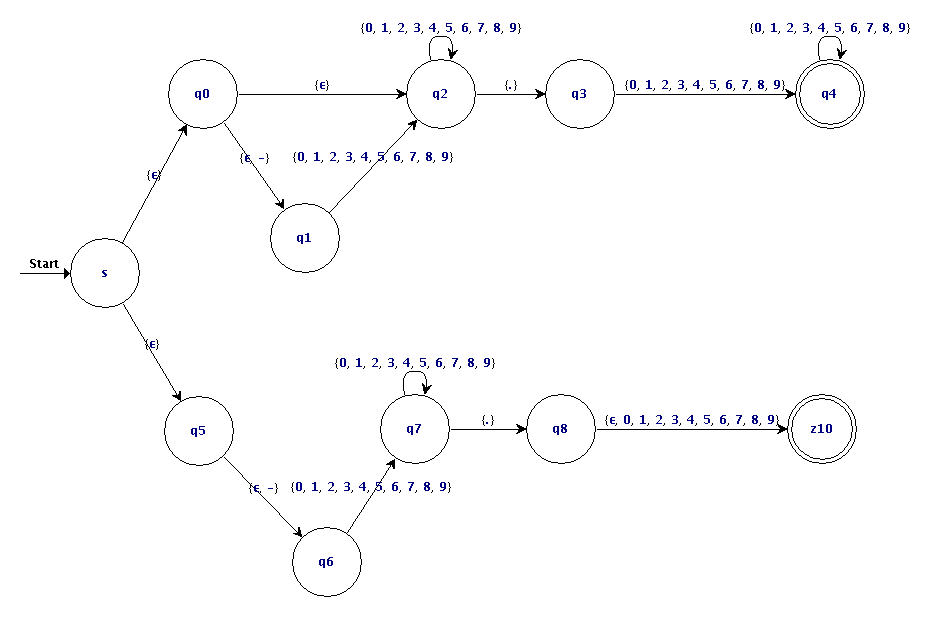
\includegraphics[width=12cm]{../images/enfa_example.png}
\end{center}
\end{figure}

\section{Neue Automat Datei anlegen}

Am Anfang müssen wir dazu erst einmal den "`Neu\ldots"' Dialog öffnen. Dort
wählen wir aus, dass wir einen Automaten erstellen wollen und klicken
auf "`Weiter"'.\vspace{10pt}

Im nächsten Dialog werden wir gefragt, von welchem Typ unser neuer
Automat sein soll. In unserem Beispiel handelt es sich um einen
"`$\epsilon$-NDEA"', welchen wir auswählen und mit "`Weiter"'
bestätigen.\vspace{10pt}

Dann müssen wir das gewünschte Alphabet für den neuen Automaten
angeben. Im Alphabet können alle Symbole werwendet werden, die nicht zur Syntax
der Eingabe gehören. Das bedeutet \Symbol{,}, \Symbol{\{}, \Symbol{\}} und
\SymbolEmpty{} können hier nicht verwendet werden. Symbole, welche länger als ein
Zeichen sind, müssen in Anführungszeichen angegeben werden.\vspace{10pt}

In dem Dialog sind an allen Stellen schon vordefinierte Werte eingetragen. Dabei
handelt es sich um die Vorgaben, die man als Standardwerte in den Einstellung
eingetragen hat. Wie man diese Standardwerte ändert, kann man in Kapitel
\ref{Preferences} nachlesen.\vspace{10pt}

Wir müssen noch die von uns benötigten Symbole angeben. Dazu tragen wir in das
Feld Alphabet "`\{\Symbol{0},\ \Symbol{1},\ \Symbol{2},\ \Symbol{3},\
\Symbol{4},\ \Symbol{5},\ \Symbol{6},\ \Symbol{7},\ \Symbol{8},\ \Symbol{9},\
\Symbol{-}\}"' ein. Damit haben wir alle benötigten Information eingegeben und
können den neuen Automaten durch Klick auf "`Fertig"' erstellen.\vspace{10pt}
\vspace{10pt} 

\begin{figure}[h]
\begin{center}
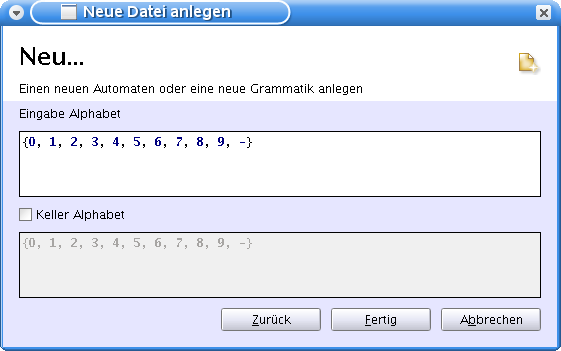
\includegraphics[width=8cm]{../images/new_dialog_machine.png}
\caption{Automat - Toolbar}
\end{center}
\end{figure}

Das für den Automaten angegebene Alphabet, lässt sich jeder Zeit über den Button
"`Dokument editieren"' nächträglich ändern.

\section{Zustände und Übergänge anlegen}

Um einen Automaten zu bearbeiten, müssen wir zuerst den entsprechenden Modus
auswählen. Folgende Modi sind in der Toolbar verfügbar:

\begin{figure}[h!]
  \begin{center}
    \begin{minipage}[t]{1cm}
      
\includegraphics[width=0.4cm]{../images/machineToolbar/mouse.png}
    \end{minipage}
    \begin{minipage}[t]{5cm}
      Maus Modus
    \end{minipage}
  \end{center}
\end{figure} 

\begin{figure}[h!]
  \begin{center}
    \begin{minipage}[t]{1cm}
      
\includegraphics[width=0.5cm]{../images/machineToolbar/state.png}
    \end{minipage}
    \begin{minipage}[t]{5cm}
      Neuer Zustand
    \end{minipage}
  \end{center}
\end{figure} 

\begin{figure}[h!]
  \begin{center}
    \begin{minipage}[t]{1cm}
      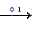
\includegraphics[width=0.5cm]{../images/machineToolbar/transition.png}
    \end{minipage}
    \begin{minipage}[t]{5cm}
      Neuer Übergang
    \end{minipage}
  \end{center}
\end{figure} 

\begin{figure}[h!]
  \begin{center}
    \begin{minipage}[t]{1cm}
      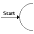
\includegraphics[width=0.5cm]{../images/machineToolbar/start.png}
    \end{minipage}
    \begin{minipage}[t]{5cm}
      Neuer Start Zustand
    \end{minipage}
  \end{center}
\end{figure}

\begin{figure}[h!]
  \begin{center}
    \begin{minipage}[t]{1cm}
      
\includegraphics[width=0.5cm]{../images/machineToolbar/final.png}
    \end{minipage}
    \begin{minipage}[t]{5cm}
      Neuer Akzeptierender Zustand
    \end{minipage}
  \end{center}
\end{figure} 


Da wir zu Beginn den Startzustand anlegen wollen, wählen wir "`Neuer Start
Zustand"' und klicken auf eine freie Fläche im unteren Teil, um den Zustand dort
zu erstellen. Um den Zustand nachträglich zu bearbeiten, müssen wir in den Maus
Modus wechseln. Den Konfigurationsdialog erreicht man dann über Doppelklick oder
das Kontextmenü. Über das Kontextmenü lässt sich ein Zustand auch wieder
löschen.\vspace{10pt}

Auf diese Weise lassen sich alle Zustände anlegen, die für den Beispielautomaten
benötigt werden. Nachdem wir alle Zustände angelegt haben, fehlen noch die
Übergänge zwischen den Zuständen. Daher wechseln wir in den "`Neuer Übergang"'
Modus. Um jetzt einen neuen Übergang anzulegen, klicken wir auf einen Zustand und
ziehen, bei gedrückter Maustaste, die Maus auf einen anderen Zustand. Beim
Loslassen öffnet sich der Konfigurationsdialog für Übergänge. In diesem Dialog
ziehen wir jetzt die Symbole, die in dem Übergang enthalten sein sollen, aus der
linken Liste mit allen Symbolen in die rechte Liste, welche die Übergangsmenge
repräsentiert. Als Hilfestellung wird im unteren Dia\-log der entstehende
Übergang angezeigt. Nach bestätigen durch "`OK"' wird der Übergang
angelegt.\vspace{10pt}

Die Übergänge lassen sich auf die gleiche Weise bearbeiten und löschen, wie es
bei den Zuständen möglich ist. Es gibt allerdings eine Besonderheit: Wenn man die
Maus anstatt über einem Zustand, über einem leeren Bereich los lässt, entsteht
beim Anlegen des Übergangs zusätzlich ein neuer Zustand.\vspace{10pt}

Diesen Vorgang wiederholen wir jetzt für alle Übergänge, die
für den Beispielautomaten benötigt werden. Wenn wir damit fertig sind, können
wir den Automaten noch validieren, um zu sehen, ob uns beim Anlegen der Zustände
und Übergänge irgendwelche Fehler unterlaufen sind. Diese Funktion erreicht man
über das Kontextmenü oder über den Menüpunkt "`Ausführen"'.\vspace{10pt}

Sollten die Zustände nicht ganz so optimal platziert sein, kann man
versuchen, über die Auto-Layout Funktion ein besseres Ergebnis zu
erreichen. Diese ist über "`Ausführen"' und "`Auto Layout"' oder über
das Kontextmenü erreichbar.

\section{Was fange ich mit einem Automaten an?}

Für einen erstellten Automaten gibt es folgende
Ver\-wen\-dungs\-möglich\-keiten.


\subsection{Bearbeiten per Übergangstabelle}

Die Übergänge eines Automaten können über die Tabelle bearbeitet werden. Diese
ist im rechten Teil des Fensters zu finden. Es ist möglich, neue Übergänge
anzulegen. Bestehende Übergänge können gelöscht oder editiert werden.\vspace{10pt}

Betrachten wir ein einfaches Beispiel. Wir legen zwei Zustände \State{z0} und
\State{z1} an und arbeiten auf dem Alphabet \{\Symbol{0}, \Symbol{1}\}. Die
Übergangstabelle besteht somit aus vier Spalten, in der ersten Spalte werden die
Zustände dargestellt, in der zweiten die Übergänge mit \Symbol{$\epsilon$} und in
den anderen die Symbole des Alphabets, also in unserem Fall je eine Spalte für
\Symbol{0} und \Symbol{1}.\vspace{10pt}

Um von \State{z0} nach \State{z1} einen $\epsilon$-Übergang anzulegen, muss die
erste Zeile mit \State{z0} bearbeitet werden. Da ein $\epsilon$-Übergang angelegt
werden soll, muss die zweite Spalte bearbeitet werden. Um dies umzusetzen, muss
auf die entsprechende Zelle doppelt geklickt werden. Es steht ein Parser zur
Verfügung, in den mit Komma getrennte Zustände eingetragen werden können. Die
Zustände müssen vorhanden sein. In userem Beispiel tragen wir also in der zweiten
Spalte, in der ersten Zeile den Zustand \State{z1} ein und bestätigen die Eingabe
mit Enter. Es wird, wie erwartet, ein $\epsilon$-Übergang von \State{z0} nach
\State{z1} angelegt.\vspace{10pt}

\begin{figure}[h]
\begin{center}
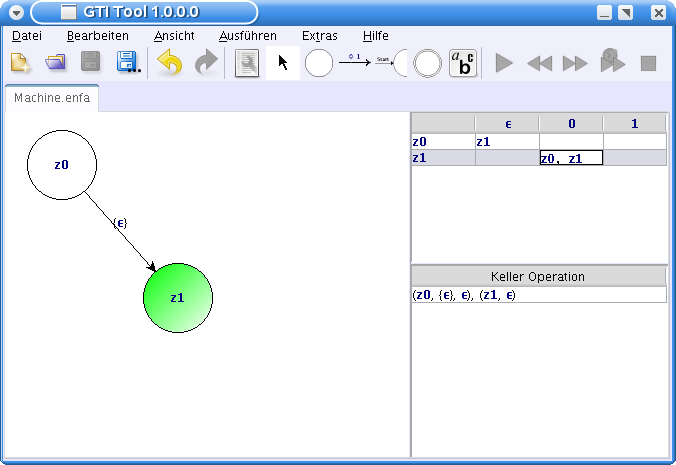
\includegraphics[width=12cm]{../images/machine_table.png}
\caption{Automat - Übergangstabelle bearbeiten}
\end{center}
\end{figure}

Als nächstes sollen zwei Übergänge auf einmal mit Symbol \Symbol{0} angelegt
werden. Beide sollen von Zustand \State{z1} ausgehen, der erste soll bei
\State{z0} enden, der zweite bei \State{z1}. Um dies umzusetzen, muss die Zeile
von \State{z1} und die Spalte von \Symbol{0} bearbeitet werden. Da der Übergang
zu den beiden Zuständen gehen soll, muss \State{z0}, \State{z1} eingetragen
werden.\vspace{10pt}

Das Löschen und Erweitern von Übergängen erfolgt analog.


\subsection{Vorlage für\ldots}
  
  Ein Automat kann als Vorlage für einen neuen Automaten benutzt werden. Dies
  sollte nicht mit "`Umwandeln in\ldots"' verwechselt werden. Es wird eine neue
  Datei angelegt, die alle Zustände und Übergänge des Ausgangsautomaten enthält.
  Allerdings kann man den Automatentypen neu festlegen.
  
\subsection{Wort-Navigation}
  
  Wir können für einen Automaten eine Wort-Navigation starten. Das bedeutet,
  dass wir ein Wort eingeben können, welches wir den Automaten verarbeiten lassen
  wollen und können dann schrittweise vor und zurück navigieren. Dabei werden
  die aktuell aktiven Zustände und Übergänge farblich hervorgehoben. Am Ende
  können wir dann sehen, ob der Automat das von uns gewählte Wort akzeptiert oder
  nicht. Dies wird über ein Statusfeld im unteren Fenster signalisiert. Es gibt
  auch die Möglichkeit, zu erkennen, ob ein Wort zu einem früheren Zeitpunkt der
  Navigation akzeptiert würde. Dies kann man anhand eines Rahmens um das aktuelle
  Wort Feld erkennen. Ein roter Rahmen steht dafür, dass das Wort bis zum
  aktuellen Symbol von unserem Automat nicht akzeptiert wird, ein grüner Rahmen
  hingegen gibt zu verstehen, dass es akzeptiert wird.\vspace{10pt}
  
  \newpage
  Während man sich im Wort-Navigations-Modus befindet, lässt sich der Automat
  nicht weiter bearbeiten. Das bedeutet, wir können Zustände und Übergänge weder
  anlegen noch löschen oder bearbeiten. Dies ist erst nach Verlassen dieses
  Modus wieder möglich.\vspace{10pt}
  
  \begin{figure}[h]
  \begin{center}
  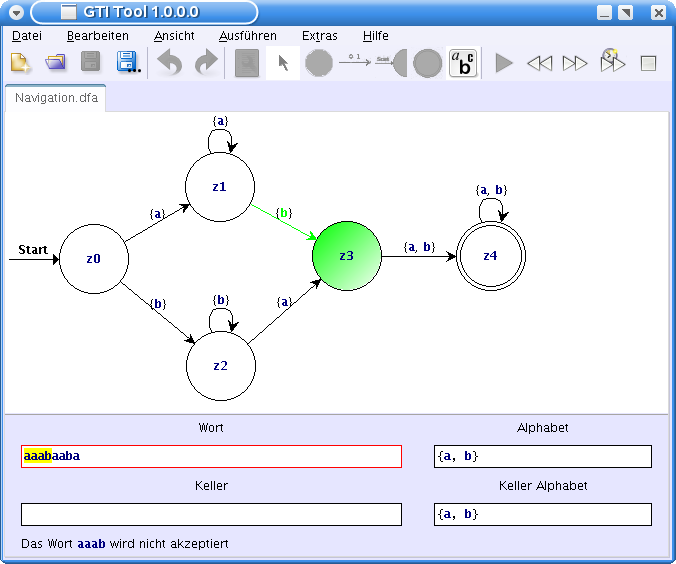
\includegraphics[width=12cm]{../images/dfa_navigation.png}
  \caption{Automat - Wort-Navigation}
  \end{center}
  \end{figure}
  
  Zur Wort-Navigation gelangt man über den Menüpunkt "`Ausführen"' und "`Wort
  eingeben"' oder direkt über den Button in der Toolbar. In dem Feld
  "`Wort"' können wir jetzt ein Wort eingeben. Als Hilfestellung sehen
  wir rechts neben dem Eingabefeld das aktuelle Alphabet mit den gültigen
  Symbolen.\vspace{10pt}
  
  Nachdem wir das Wort eingegeben haben, startet man die Navigation über
  "`Start"' in der Toolbar oder im Kontextmenü. Jetzt kann man mit "`Schritt vor"' und
  "`Schritt zurück"' durch das Wort navigieren. Es existiert auch noch ein
  automatischer Modus. Dabei wird nach einer kurzen Verzögerung das nächste
  Symbol gelesen. Dieser Modus lässt sich durch den Button "`Automatische
  Schritte"' aktivieren und deaktivieren.\vspace{10pt}

  \newpage
  Wenn man wissen möchte, über welche Pfade man zu den momentan aktiven Zuständen
  gelangt ist, kann man sich dies über "`Extras"' und "`Zustands Pfad"' anzeigen
  lassen. Es öffnet sich ein neuer Dialog mit einer Tabelle, in welcher für
  jeden aktiven Zustand der aktuelle Pfad angezeigt wird. Dabei wird als erstes der
  kürzeste Pfad angezeigt, und dann alle weiteren.\vspace{10pt}
  
    \begin{figure}[h]
  \begin{center}
  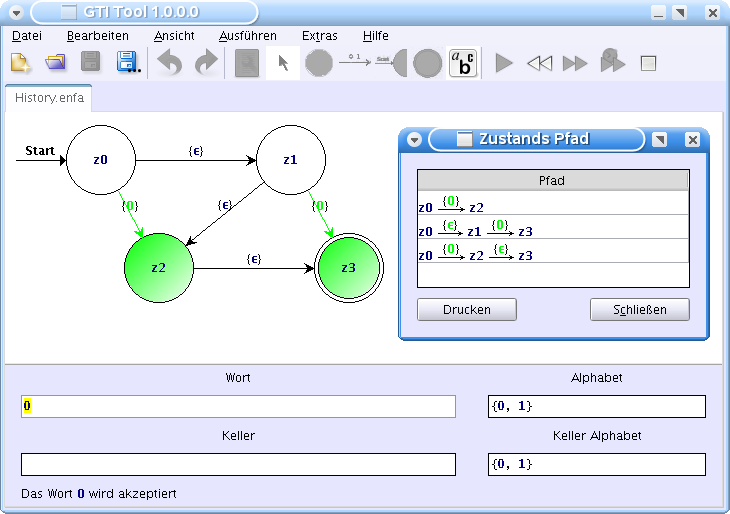
\includegraphics[width=12cm]{../images/history_path.png}
  \caption{Automat - Minimieren}
  \end{center}
  \end{figure}
  
  Um die Wort-Navigation zu beenden, klickt man einfach wieder auf den Button
  "`Wort eingeben"' in der Toolbar oder man wählt im Menü "`Ausführen"' den
  Punkt "`Automat bearbeiten"'. Jetzt befinden wir uns wieder im normalen Modus
  und wir können den Automaten wieder normal bearbeiten.
   
\subsection{Minimieren}
  
  Es besteht auch die Möglichkeit sich aus einem DFA den minimalen Automaten
  berechnen zu lassen. Für diese Funktion darf der Automat allerdings keine
  Fehler mehr enthalten, was wir durch eine Validierung ausschließen können. Das
  Minimieren startet man über den Menüpunkt "`Ausführen"' und
  "`Minimieren"'.\vspace{10pt}
  
  Es öffnet sich ein neuer Dialog mit einer Ansicht des Automaten und einer
  Tabelle. Der Automat sieht im Moment noch genau wie unser Ausgangsautomat
  aus. Wenn man allerdings jetzt auf "`Schritt vor"' klickt, werden als erster
  Schritt alle nicht erreichbaren Zustände entfernt. In der Outline wird
  angegeben, um welche Zustände es sich dabei handelt. Der zweite Schritt
  besteht darin, die erste Einteilung der Äquivalenzklassen vorzunehmen. Dazu
  unterteilen wir die Zustände des Automaten in akzeptierende und nicht
  akzeptierende Zustände. In der Automatenansicht werden immer die Zustände in
  der selben Farbe dargestellt, welche sich in einer Äquivalenzklasse befinden.
  Jetzt haben alle nicht akzeptierenden Zustände die gleiche Farbe. Gleiches 
  gilt für alle akzeptierenden Zustände, welche natürlich in einer anderen
  Farbe dargestellt werden.\vspace{10pt}
  
  \begin{figure}[h!]
  \begin{center}
  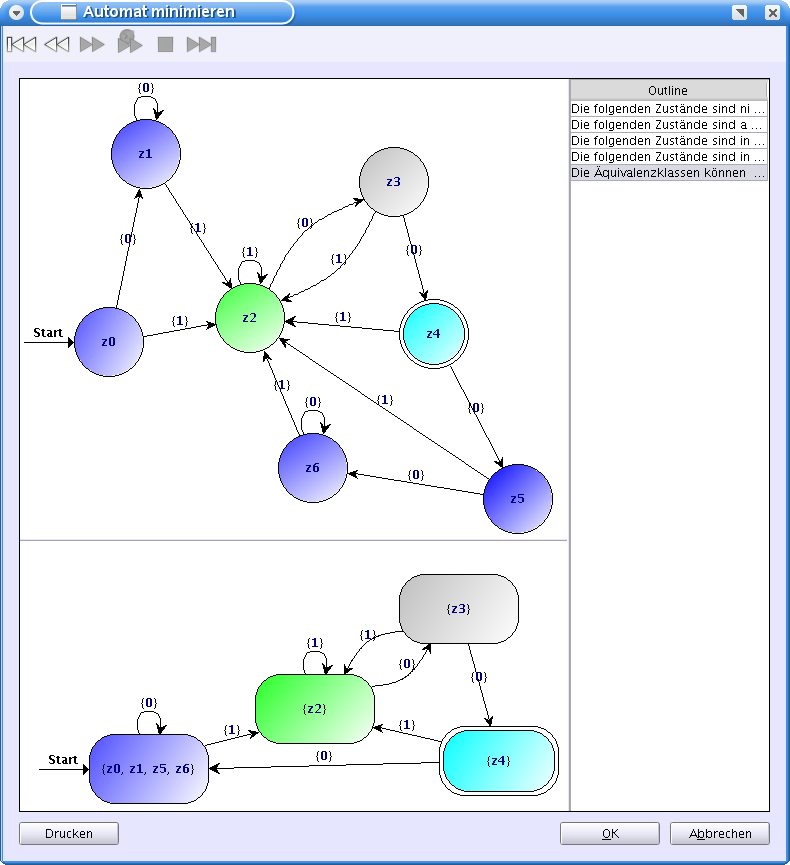
\includegraphics[width=12cm]{../images/minimize.png}
  \caption{Automat - Minimieren}
  \end{center}
  \end{figure}
  
  \newpage
  Man kann jetzt durch Klicken auf "`Schritt vor"' die Äquivalenzklassen weiter
  verfeinern. In der Outline wird angegeben, welche Zustände in eine eigene
  Äquivalenzklasse gekommen sind, und diese werden jetzt auch in einer anderen
  Farbe dargestellt. Gleichzeitig werden auch die Übergänge hervorgehoben, welche
  bei diesem Verfeinerungsschritt eine Rolle gespielt haben. Dabei beziehen sich
  die hervorgehobenen Übergänge immer auf den aktuell ausgewählten
  Tabelleneintrag.\vspace{10pt}
  
  Auf diese Weise kann man den Automaten jetzt Schritt für Schritt weiter
  verfeinern, bis keine Verfeinerung der Äquivalenzklassen mehr möglich ist. Wenn
  das der Fall ist, wird auch eine zweite Automatenansicht eingeblendet, dem
  entstandenen minimierten Automaten. Durch bestätigen mit "`OK"' wird jetzt
  eine neue Datei mit dem minimierten Automaten erstellt, mit welchem man dann
  weiter arbeiten kann.\vspace{10pt}
  
  Natürlich kann der Minimierungsprozess jederzeit abgebrochen werden. In diesem
  Fall wird keine neue Datei angelegt, man kann den Ausgangsautomaten weiter
  bearbeiten. \vspace{10pt}
  
  Wenn man in den Navigationsbereich des Dialogs schaut, stellt man fest, dass
  noch weitere Button verfügbar sind, auf welche jetzt noch nicht eingegangen
  wurde. Zunächst einmal gibt es die Button "`Bis zum Ende vor"' und "`An den
  Anfang zurück"'. Mit "`Bis zum Ende vor"' kann man alle Zwischenschritte
  überspringen, und gelangt direkt zur Ansicht des minimalen Automaten. "`An den
  Anfang zurück"' bewirkt genau das Gegenteil, und springt zur Ausgangsansicht
  zurück. Dann gibt es noch einen "`Schritt zurück"' Button, welcher einzelne
  Verfeinerungsschritte rückgängig macht. Und schlussendlich gibt es noch einen
  Button "`Automatische Schritte"', welcher nach einer kurzen Verzögerung
  automatisch den nächsten Schritt macht, bis der Minimierungsprozess
  abgeschlossen ist. Diese Funktion kann durch den "`Stop"' Button wieder
  deaktiviert werden.\vspace{10pt}
  
  Wenn man die neue Datei mit dem minimalen Automaten erstellen möchte, ohne sich
  die Minimierung im Detail anzuschauen, besteht jederzeit die Möglich\-keit,
  den Dialog mit "`OK"' zu bestätigen. Die Minimierung wird dann im Hintergrund
  beendet, man gelangt sofort zur Ansicht des neu entstandenen Automaten und
  kann mit diesem weiterarbeiten.
  
  
\subsection{Umwandeln in\ldots}\label{ConvertTo}
  
Es besteht auch die Möglichkeit, zwischen verschiedenen Automatentypen
umzuwandeln. Dabei stehen drei Umwandlungen zur Verfügung, die sich in den
verwendeten Schritten unterscheiden.

\begin{itemize}
  \item NDEA $\to$ DEA
  \item $\epsilon$-NDEA $\to$ DEA
  \item $\epsilon$-NDEA $\to$ NDEA
\end{itemize}

Betrachten wir als erstes einen einfachen NDEA mit zwei Zuständen \State{z0} und
\State{z1} und zwei Übergängen, der auf dem Alphabet \{\Symbol{a}, \Symbol{b}\}
arbeitet. Der Zustand \State{z0} ist ein Start-Zustand, der Zustand \State{z1}
ein akzeptierender Zustand. Der erste Übergang besteht zwischen \State{z0} und
\State{z1} mit Symbol \Symbol{a}, der zweite geht von \State{z0} in sich selbst
über, ebenfalls mit \Symbol{a}. Der Automat erkennt somit Wörter von der Form
$a^n$ für $n \geq 1$. Über den Eintrag "`Umwandeln in\ldots"' im Menüeintrag
"`Ausführen"' kann ausgewählt werden, in welchen Automaten umgewandelt wird. Da
wir einen NDEA angelegt haben, ist hier nur der DEA verfügbar. Wird dieser
ausgewählt, steht die schon aus anderen Ansichten bekannte Oberfläche zur
Verfügung. Auch hier kann in einzelnen Schritten, sowie automatisch navigiert
werden. Wird der Dialog mit "`OK"' bestätigt, steht in der Hauptansicht der
umgewandelte Automat zur Verfügung. Mit "`Abbrechen"' wird der Dialog einfach nur
geschlossen.\vspace{10pt}

\begin{figure}[h!]
\begin{center}
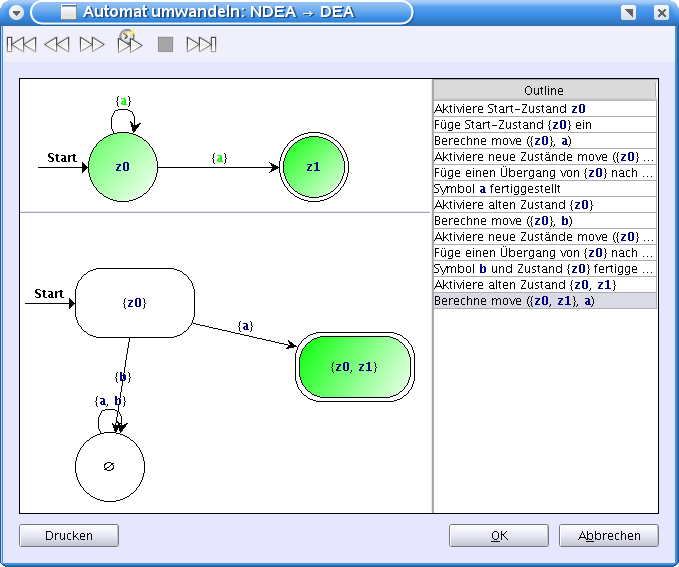
\includegraphics[width=12cm]{../images/convert_to.png}
\caption{Automat - Umwandeln in\ldots}
\end{center}
\end{figure}

\newpage
Werden die Schritte einzeln durchgegangen, ergibt sich folgender Ablauf:

\begin{enumerate}
  \item Der Start-Zustand \State{z0} wird aktiviert.
  \item In der unteren Ansicht wird der Start-Zustand \{\State{z0}\} angelegt.
  \item Die Übergänge mit dem ersten Symbol aus dem Alphabet, also \Symbol{a},
  werden hervorgehoben, um anzuzeigen, welche Zustände mit dem Symbol zu
  erreichen sind.
  \item In unserem Beispiel sind das die Zustände \State{z0} und \State{z1},
  die hervorgehoben werden.
  \item In der unteren Ansicht wird ein Übergang von \{\State{z0}\} nach
  \{\State{z0}, \State{z1}\} mit Symbol \Symbol{a} angelegt. Da dieser zweite
  Zustand in unserem Beispiel noch nicht existiert, wird er angelegt.
  \item Dieser Schritt zeigt an, dass das Symbol \Symbol{a} fertiggestellt ist.
  \item Da für den Zustand \{\State{z0}\} noch nicht alle Symbole betrachtet
  wurden, wird er aktiviert.
  \item Es wird die gleiche Berechnung wie bei Schritt drei durchgeführt,
  allerdings für Symbol \Symbol{b}. Da es in unserem Beispiel keinen Übergang
  von den betroffen Zuständen, bei uns nur \State{z0}, gibt, werden in der
  oberen Ansicht keine Übergänge hervorgehoben.
  \item Wie in Schritt vier werden die mit Symbol \State{b} erreichbaren
  Zustände in der oberen Ansicht hervorgehoben. In unserem Beispiel existiert
  kein Übergang von \State{z0} mit Symbol \Symbol{b}, deshalb werden in der
  oberen Ansicht keine Zustände hervorgehoben.
  \item Da wir in diesem Beispiel in einen DEA umwandeln, wird auch für diesen
  Fall ein Zustand angelegt und zwar der nicht akzeptierende Zustand
  \State{$\emptyset$}. Wird dieser Zustand während der Wort-Navigation
  erreicht, kann das Wort nicht mehr akzeptiert werden. Aus diesem Grund wird
  direkt der Übergang von diesem Zustand in sich selbst mit allen Symbolen des
  Alphabets angelegt. Es wird ein Übergang mit Symbol \Symbol{b} zu diesem
  Zustand \State{$\emptyset$} angelegt.
  \item Wie in Schritt sechs wird angezeigt, dass das Symbol \Symbol{b} fertig
  verarbeitet wurde. Da dieses Symbol das letzte im Alphabet ist, ist der
  Zustand \{\State{z0}\} fertiggestellt.
  \item In diesem Schritt wird der nächste, bis jetzt noch nicht verarbeitete,
  Zustand \{\State{z0}, \State{z1}\} in der unteren Ansicht hervorgehoben.
  Gleichzeitig werden in der oberen Ansicht die entsprechenden Zustände
  \State{z0} und \State{z1} hervorgehoben.
  \item Es folgt wieder das Hervorheben der Übergänge mit dem Symbol
  \Symbol{a}, wie dies in Schritt drei der Fall war.
  \item Wie in Schritt vier werden die Zustände \State{z0} und \State{z1}
  hervorgehoben.
  \item In Schritt fünf wurde der Übergang zum Zustand \{\State{z0},
  \State{z1}\} mit Symbol \Symbol{a} angelegt, gleiches geschieht jetzt in
  diesem Schritt. Da wir allerdings im Moment den gleichen Zustand bearbeiten,
  wird der Übergang von diesem Zustand in sich selbst angelegt.
  \item Das Symbol \Symbol{a} ist fertiggestellt.
  \item Da der Zustand \{\State{z0}, \State{z1}\} noch nicht fertiggestellt
  ist, wird er in beiden Ansichten wie gehabt hervorgehoben.
  \item Alle Übergänge, die von den Zuständen \State{z0} und \State{z1} mit
  Symbol \Symbol{b} ausgehen, werden hervorgehoben. In unserem Beispiel kommt
  das nicht vor.
  \item Die mit dem Symbol \Symbol{b} erreichbaren Zustände werden
  hervorgehoben, in unserem Beispiel ist das wieder kein Zustand.
  \item Deshalb wird in diesem Schritt wieder ein Übergang mit Symbol
  \Symbol{b} zu dem Zustand \State{$\emptyset$} angelegt.
  \item Der Zustand \{\State{z0}, \State{z1}\} ist mit dem letzten Symbol
  \Symbol{b} fertiggestellt. Da keine weiteren Zustände hinzugekommen sind, ist
  die Umwandlung fertiggestellt.
\end{enumerate}

Bei Betrachten des entstehenden DFA's erkennt man, dass dieser die gleichen
Wörter erkennt wie der ursprüngliche NFA. Der Dialog kann mit "`OK"' bestätigt
werden, womit ein neuer DFA angelegt wird. Es ist jetzt möglich, die Namen der
Zustände neu zu vergeben, wenn man mit dem Automaten weiterarbeiten möchte und
nicht die längeren Namen dargestellt haben möchte. Dazu kann man im Menü
"`Extras"' den Eintrag "`Zustandsnamen neu vergeben"' anklicken, wodurch die
Zustandsnamen neu, nach dem Muster \State{z0}, \State{z1} \ldots, vergeben
werden.\vspace{10pt}

Zu den anderen zwei Umwandlungarten gibt es noch kleinere Änderungen, die bei dem
durchgespielten Beispiel nicht betrachtet werden konnten. Wird ein
$\epsilon$-NDEA in einen NDEA umgewandelt, entfällt das Anlegen des Zustandes
\State{$\emptyset$}, es wird einfach kein Übergang mit dem entsprechenden Symbol
angelegt, da bei einem NFA nicht alle Symbole vorhanden sein
müssen.\vspace{10pt}

Wird ein $\epsilon$-NDEA umgewandelt, kommen jeweils zwei Schritte dazu. So wird
nach dem Aktivieren der alten Zustände, bei unserem Beispiel die Schritte eins,
sieben, etc., der $\epsilon$-Abschluss berechnet, es werden also auch alle
Zustände aktiviert, die mit $\epsilon$-Übergängen zu erreichen sind. Gleiches
gilt für das Anzeigen der neuen Zustände, bei unserem Beispiel in den Schritten
vier, neun etc., auch hier werden in einem einzelnen Schritt alle Zustände
hervorgehoben, die mit $\epsilon$-Übergängen zu erreichen sind.


\subsection{Umwandeln in\ldots (Potenzmenge)}
Der einzige Unterschied zwischen den Menüpunkten "`Umwandeln in\ldots"' und
"`Umwandeln in\ldots (Potenzmenge)"' ist, dass alle Zustände bei Verwendung der
Potenzmenge bereits zu Beginn angelegt werden, auch solche, die nicht benötigt
werden, die also nicht erreichbar sind. In dem in Abschnitt \ref{ConvertTo}
gewählten Beispiel wäre das der Zustand \{\State{z1}\}, da dieser nicht zu
erreichen ist und nur einen Übergang mit allen Symbolen zu dem Zustand
\State{$\emptyset$} hat. Wie solche Zustände im Anschluss entfernt werden können,
kann im Abschnitt \ref{ReachableStates} nachgelesen werden.


\subsection{Umwandeln in Regulären Ausdruck}

Es besteht die Möglichkeit einen DFA in einen Regulären Ausdruck umzuwandeln.
Dazu betrachten wir den Beispielautomat aus der Vorlesung:

\begin{figure}[h]
\begin{center}
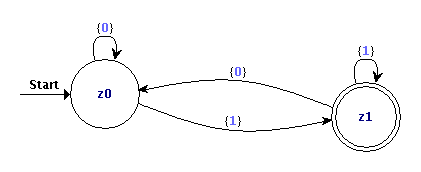
\includegraphics[width=12cm]{../images/dfa_for_regex.png}
\end{center}
\end{figure}

Für diesen Beispielautomat liefe der Algorithmus wie folgt ab:

\begin{itemize}

   \item Zunächst wird ein Ausdruck für den gesamten Automaten angelegt. In unserem Fall wurde $L_{z_0 z_1}^3 = L_{z_0 z_1}^2 | L_{z_0 z_1}^2 · (L_{z_1 z_1}^2)* · L_{z_1 z_1}^2$ angelegt.
   \item Nun werden die einzelnen Sprachen konkretisiert. In unserem Beispiel zunächst $L_{z_0 z_1}^2$. Dies wird in $L_{z_0 z_1}^1 | L_{z_0 z_0}^1 · (L_{z_0 z_0}^1)* · L_{z_0 z_1}^1$ umgewandelt.
   \item Im nächsten Schritt wird dann $L_{z_0 z_1}^1$ in \Symbol{1} umgewandelt.
   \item Dies wird solange fortgesetzt bis alle Sprachen zu Regulären Ausdrücken umgewandelt sind.
   \item In unserem Fall ist das Ergebnis $((1|(0|\epsilon)(0|\epsilon)*1)|(1|(0|\epsilon)(0|\epsilon)*1)((1|\epsilon)|0(0|\epsilon)*1)*((1|\epsilon)|0(0|\epsilon)*1))$

\end{itemize}

\begin{figure}[h!]
\begin{center}
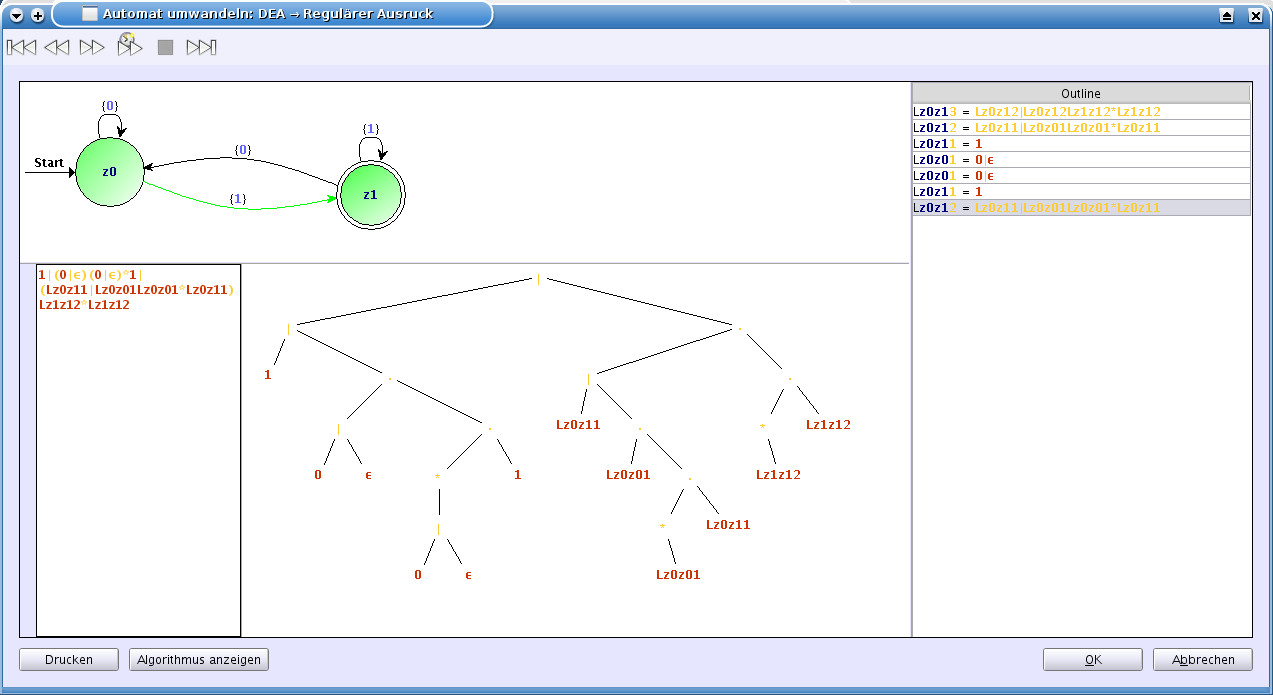
\includegraphics[width=12cm]{../images/dfa_to_regex.png}
\caption{Automat - Umwandeln in Regulären Ausdruck}
\end{center}
\end{figure}

\paragraph{Achtung:} Wie im Beispiel zu sehen, wird der Reguläre Ausdruck selbst bei einem kleinen Automaten schon relativ groß. Daher ist bei größeren Automaten mit erheblichem Rechenaufwand zu rechnen.

\subsection{Erreichbare Zustände}\label{ReachableStates}

Über den Menüeintrag "`Extras"' kann der Punkt "`Erreichbare Zustände"'
ausgewählt werden. In dem erscheinenden Dialog kann, wie in den anderen auch,
durch die einzelnen Schritte navigiert werden. Es geht hierbei darum, in
möglichst kleinen Schritten zu erkennen, welche Zustände erreichbar sind und
welche nicht. Der verwendete Algorithmus geht dabei in folgenden drei Schritten
vor:

\begin{itemize}
  \item Ein Zustand, der noch nicht berechnet wurde, wird ausgewählt (am Anfang
  wird mit dem Start Zustand begonnen)
  \item Die von dem ausgewählten Zustand aus zu erreichenden Zustände werden
  hervorgehoben, und falls sie noch nicht berechnet wurden, zu der Menge der
  noch zu berechnenden Zustände hinzugefügt
  \item Die bis jetzt erreichbaren Zustände werden hervorgehoben. Die Menge der
  noch nicht berechneten Zustände angezeigt 
\end{itemize}

\begin{figure}[h!]
\begin{center}
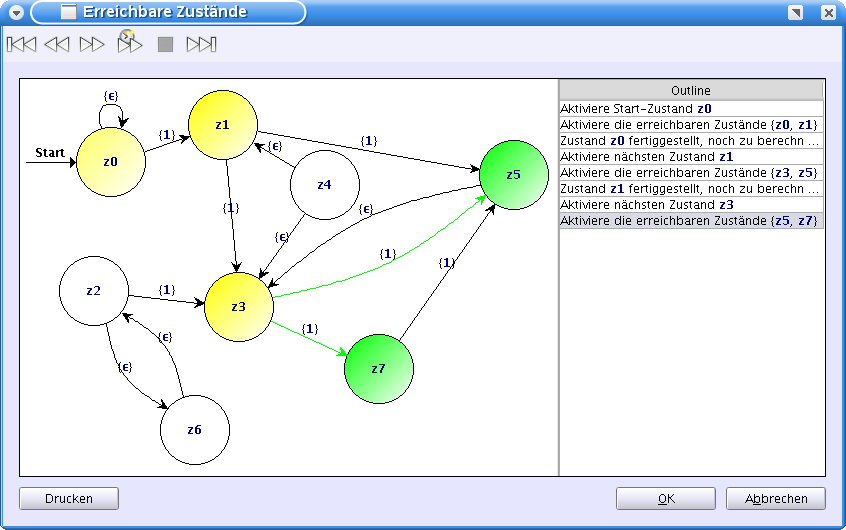
\includegraphics[width=12cm]{../images/reachable_states.png}
\caption{Automat - Erreichbare Zustände}
\end{center}
\end{figure}

Der Algorithmus läuft so lange, bis die Menge der noch nicht berechneten Zustände
leer ist. Am Ende werden alle erreichbaren Zustände farblich hervorgehoben. Wie
in den anderen Dialogen besteht jederzeit die Möglichkeit, den Dialog
abzubrechen, wobei er dann einfach geschlossen wird. Man hat auch jederzeit die
Möglichkeit, mit einem Klick auf "`OK"' die komplette Berechnung durchzuführen
und einen Automaten anzulegen, der nur noch die erreichbaren Zustände enthält.


%%
%% $Id$
%%
%% Copyright (c) 2007-2009 Christian Fehler
%% Copyright (c) 2007-2009 Benjamin Mies
%%


\chapter{Grammatiken}\label{Grammar}

Folgende Grammatik soll uns im Folgenden als Beispiel dienen:
\vspace{10pt}

\begin{tabular}{lcr}
G = ($\Sigma, N, S, P )\ mit $\\
$\Sigma = \{\TerminalSymbol{0}, \TerminalSymbol{1}, \TerminalSymbol{x},
\TerminalSymbol{y}, \TerminalSymbol{-}, \TerminalSymbol{+},
\TerminalSymbol{*}, \TerminalSymbol{(}, \TerminalSymbol{)}\}$\\ $N =
\{\StartSymbol{E}\}$\\ $S=\StartSymbol{E}$\\
$P = \{\StartSymbol{E} \to \TerminalSymbol{0},\ \StartSymbol{E} \to \TerminalSymbol{1},\
\StartSymbol{E}	\to \TerminalSymbol{x},\ \StartSymbol{E} \to \TerminalSymbol{y},\
\StartSymbol{E} \to (\TerminalSymbol{-}\StartSymbol{E}),$\\
$\ \ \ \ \ \ \ \ \StartSymbol{E} \to (\StartSymbol{E} \TerminalSymbol{+}
\StartSymbol{E}),\ \StartSymbol{E} \to (\StartSymbol{E} \TerminalSymbol{-} \StartSymbol{E}),\
\StartSymbol{E} \to (\StartSymbol{E} \TerminalSymbol{*} \StartSymbol{E})\}$\\
\end{tabular}

\section{Neue Grammatik-Datei anlegen}

Am Anfang müssen wir dazu erst einmal den "`Neu\ldots"'-Dialog öffnen. Zu finden
ist dieser in der Toolbar oder im Menüeintrag "`Datei"'. Dort wählen wir aus,
dass wir eine Grammatik erstellen wollen und klicken auf "`Weiter"'.\vspace{10pt}

Im nächsten Dialog werden wir gefragt, von welchem Typ unsere neue Grammatik
sein soll. In unserem Beispiel handelt es sich um eine "`Kontextfreie
Grammatik"', welche wir auswählen und mit "`Weiter"' bestätigen.\vspace{10pt}

Als nächstes müssen wir die benötigten Nichtterminalzeichen (N),
Terminalzeichen ($\Sigma$) und das Startzeichen (S) angeben.  Als Zeichen
können alle Symbole werwendet werden, die nicht zur Syntax der Eingabe gehören.
Das bedeutet \Symbol{,}, \Symbol{\{}, \Symbol{\}}, \Symbol{$\vert$} und \SymbolEmpty{}
können hier nicht verwendet werden. Symbole, welche länger als ein Zeichen sind,
müssen in Anführungszeichen angegeben werden.\vspace{10pt}

In dem Dialog sind an allen Stellen schon vordefinierte Werte eingetragen.
Dabei handelt es sich um die Vorgaben, die man als Standardwerte in den
Einstellungen eingetragen hat.

Wie man diese Standardwerte ändert, kann man in Kapitel \ref{Preferences}
nachlesen. Wir tragen jetzt als erstes die von uns benötigten
Nichtterminalzeichen ein. Dabei handelt es sich bei uns lediglich um das Symbol
\StartSymbol{E}. Also schreiben wir in das Feld
"`\{\StartSymbol{E}\}"'.\vspace{10pt}

Nun legen wir das Startzeichen fest. Das ist bei uns das \StartSymbol{E},
welches wir in das Feld für das Startzeichen schreiben.\\
Zum Schluss müssen wir noch die Terminalzeichen festlegen. Dazu tragen
wir in das entsprechende Feld "`\{\TerminalSymbol{0}, \TerminalSymbol{1},
\TerminalSymbol{x}, \TerminalSymbol{y}, \TerminalSymbol{+},
\TerminalSymbol{*}, \TerminalSymbol{(}, \TerminalSymbol{)}\}"' ein.\\ Damit
haben wir alle benötigten Informationen eingegeben und können die neue Grammatik
durch Klick auf "`Fertig"' erstellen.\vspace{10pt}

\begin{figure}[h]
\begin{center}
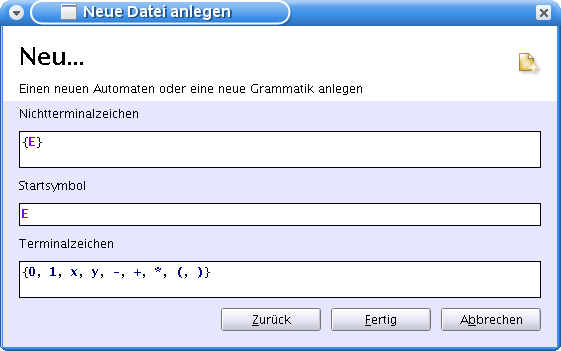
\includegraphics[width=8cm]{../images/new_dialog_grammar.png}
\caption{Grammatik - Neu Dialog}
\end{center}
\end{figure}

Alle Einstellungen, die wir gerade im letzen Dialog für die neue Datei getroffen
haben, lassen sich über "`Dokument editieren"' nachträglich ändern.

\section{Anlegen von Produktionen}

Um eine neue Produktion anzulegen, können wir den entsprechenden Button in der
Toolbar verwenden oder über den Kontextmenüeintrag gehen.\vspace{10pt}

Im Dialog für neue Produktionen müssen wir zunächst einmal angeben, für welches
Nichtterminalzeichen wir eine Produktion anlegen möchten. Dieses können wir aus
einer Liste der verfügbaren Zeichen auswählen. Da wir in unserem Beispiel nur
ein Nichtterminalzeichen haben, ist schon das richtige ausgewählt, und wir
können diesen Schritt überspringen.\vspace{10pt}

Jetzt müssen wir noch das Produktions-Wort angeben. Als Hilfestellung wird in
dem Dialog angezeigt, welche Nichtterminalzeichen und Terminalzeichen uns zur
Verfügung stehen. Wir fangen an mit der Produktion "`$\StartSymbol{E} \to
(\StartSymbol{E} \TerminalSymbol{+} \StartSymbol{E})$"'. Also geben wir als
Produktions Wort "`(\StartSymbol{E} \TerminalSymbol{+} \StartSymbol{E})"' ein.
Als weitere Hilfestellung wird im unteren Dialog die resultierende Produktion im
Ganzen angezeigt. Wir bestätigen den Dialog noch mit "`OK"' und die neue
Produktion erscheint in unserer Liste.\vspace{10pt}

\begin{figure}[h]
\begin{center}
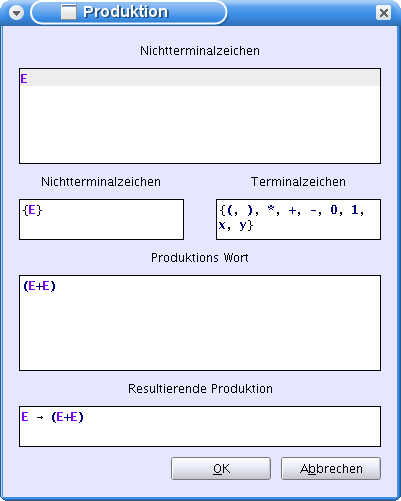
\includegraphics[width=8cm]{../images/production_dialog.png}
\caption{Grammatik - Produktionsdialog}
\end{center}
\end{figure}

Wir können die Produktion selbstverständlich auch editieren und wieder löschen.
Beide Funktionen sind über das Kontextmenü für die ausgewählte Produktion
verfügbar.\vspace{10pt}

Diesen Vorgang wiederholen wir jetzt für unsere komplette Menge "`P"'.
Alternativ k"onnen gleich mehrere Produktionen, die auf der linken Seite dasselbe
Nichterminalzeichen haben, auf einmal eingegeben werden: Die Produktionswörter müssen
in diesem Fall durch ein $\vert$ getrennt eingegeben werden. \vspace{10pt}

\newpage

\begin{figure}[h]
\begin{center}
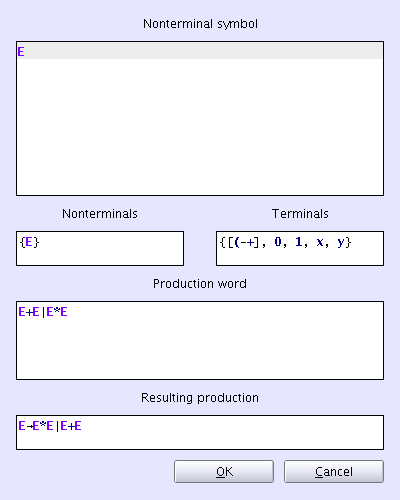
\includegraphics[width=8cm]{../images/production_dialog_multi.png}
\caption{Grammatik - Produktionsdialog}
\end{center}
\end{figure}

Wenn wir alle Produktionen angelegt haben, sind wir auch mit dem Anlegen der Grammatik
fertig. Es besteht jetzt noch die Möglichkeit, die Grammatik zu validieren, um
zu sehen, ob man beim Erstellen irgendwelche Fehler gemacht hat. Diese Funktion
erreicht man über das Kontextmenü oder über den Menüpunkt "`Ausführen"'.

\begin{figure}[h]
\begin{center}
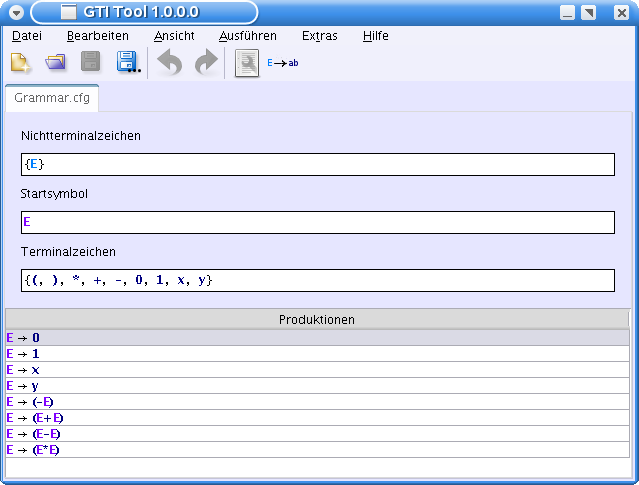
\includegraphics[width=8cm]{../images/cfg_example.png}
\caption{Grammatik - Kontextfreie Grammatik}
\end{center}
\end{figure}

\section{Umwandeln und Validieren}

Es ist zu beachten, dass beim Umwandeln einer Grammatik keine
Validierungsfehler vorhanden sein dürfen. Bei der Funktion "`Vorlage
für\ldots"' spielen Fehler allerdings keine Rolle.

\subsection{Vorlage f"ur eine andere Grammatik}
Eine Grammatik kann als Vorlage für eine neue Grammatik benutzt werden.
Das ist zum Beispiel sinnvoll, wenn wir eine kontextfreie Grammatik
haben und jetzt eine reguläre Grammatik mit den gleichen Produktionen
erstellen wollen. Dazu öffnet man den Menüpunkt "`Ausführen"' und wählt unter
"`Vorlage für\ldots"' den gewünschten Typ der neuen Datei aus.
Dabei ist zu beachten, dass die Grammatik nicht konvertiert wird,
sondern nur als Vorlage verwendet wird.\vspace{10pt}

\subsection{Umwandeln in Automaten}
Aus einer Grammatik kann der ent\-sprechen\-de Automat generiert werden.
Es besteht die Möglichkeit,
sich für eine reguläre Grammatik den entsprechenden NDEA, und für eine
kontextfreie Grammatik den entsprechenden Kellerautomaten, LR0-Automaten und
LR1-Automaten erzeugen zu lassen. Zu finden ist die Umwandlung im Menüeintrag "`Ausführen"'
unter "`Umwandeln in\ldots"'.\vspace{10pt}

\subsection{Umwandeln in Parser}
Es können die entsprechenden Parser aus einer kontextfreien Grammatik generiert werden.
Im Menü "`Ausführen"' befindet sich der Eintrag "`Top-Down-Parser erstellen"'.
Im Untermenü "`Umwandeln in"' unter dem Menü "`Ausführen"' befinden sich die Einträge:
"`LR0-Parser erstellen"', "`LR1-Parser erstellen"', "`SLR-Parser erstellen"' und
"`LALR1-Parser erstellen"'.

\subsection{Erzeugen der FIRST- und FOLLOW-Mengen}
Zu einer kontextfreien Grammatik können die FIRST- und FOLLOW-Mengen 
berechnet werden. Hierzu wählt man im Menü "`Ausführen"' "`First-Menge berechnen"'
bzw. "`Follow-Menge berechnen"'. Danach wird ein Dialog angezeigt, in dem die
entsprechende Menge schrittweise berechnet wird, wobei links der aktuelle Fortschritt
und rechts die Gründe für das Vergrößern einer der Mengen angezeigt werden.

\begin{figure}[h]
\begin{center}
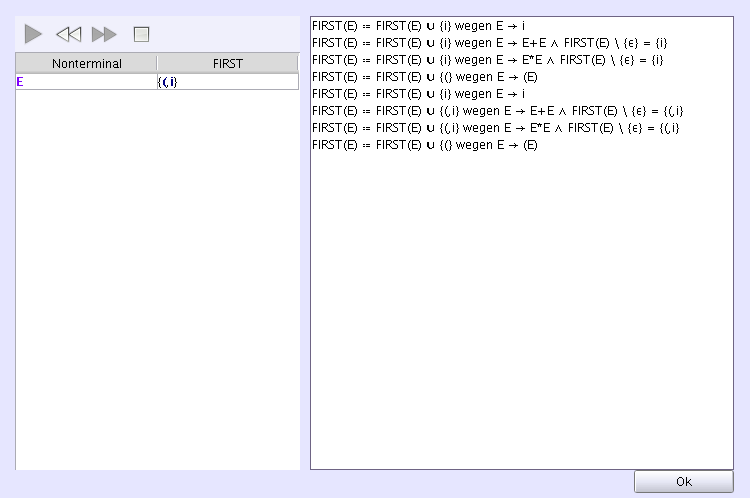
\includegraphics[width=12cm]{../images/follow.png}
\caption{Grammatik - Follow berechnen}
\end{center}
\end{figure}

\subsection{Einheitsproduktionen entfernen}

Hierzu nutzen wir die folgende Beispielgrammatik:

\begin{tabular}{lcr}
G = ($\Sigma, N, S, P )\ mit $\\
$\Sigma = \{\TerminalSymbol{a}, \TerminalSymbol{b}, \TerminalSymbol{c},
\TerminalSymbol{d}\}$\\ $N =
\{\NonterminalSymbol{A}, \StartSymbol{S}\}$\\ $S=\StartSymbol{S}$\\
$P = \{\StartSymbol{S} \to \NonterminalSymbol{A}\TerminalSymbol{a},\ \StartSymbol{S} \to \TerminalSymbol{b},\
\NonterminalSymbol{A}	\to \NonterminalSymbol{A}\TerminalSymbol{c},\ \NonterminalSymbol{A} \to \StartSymbol{S}\TerminalSymbol{d},\
\NonterminalSymbol{A} \to \epsilon, \
\NonterminalSymbol{A} \to \StartSymbol{S}\}$\\
\end{tabular}

Nun findet man im Menü unter "`Ausführen"' den Punkt "`Einheitsproduktionen entfernen"'. Es erscheint das folgende Fenster.

\begin{figure}[h]
\begin{center}
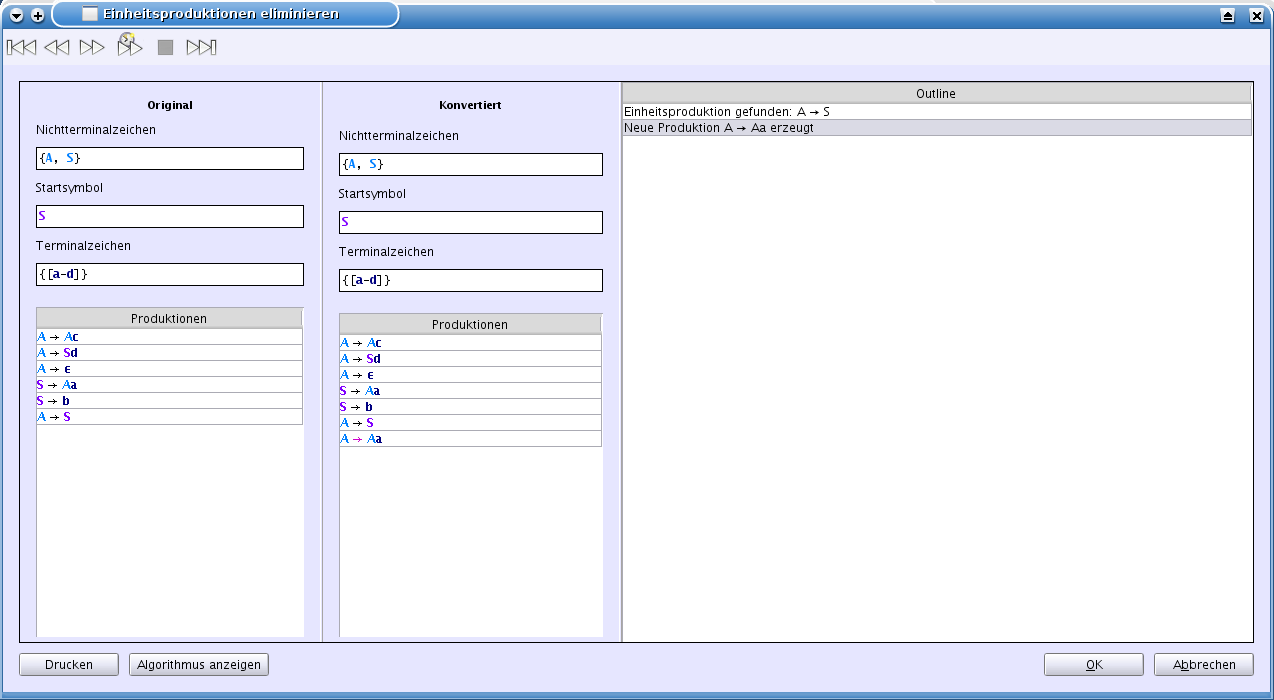
\includegraphics[width=12cm]{../images/unit_productions.png}
\caption{Grammatik - Einheitsproduktionen entfernen}
\end{center}
\end{figure}

Ganz links befindet sich die ursprüngliche Grammatik. Rechts daneben findet man die neue Grammatik. Diese ist am Anfang gleich der Ursprünglichen und wird erst im Verlauf des Algorithmus verändert.

Zunächst sucht der Algorithmus nun nach einer Einheitsproduktion und findet die Produktion $\NonterminalSymbol{A} \to \StartSymbol{S}$.

Nun wird für jede Produktion von $\StartSymbol{S}$ eine entsprechende Produktion für $\NonterminalSymbol{A}$ hinzugefügt. Dies wäre in unserem Beispiel zunächst die Produktion $\NonterminalSymbol{A} \to \NonterminalSymbol{A}\TerminalSymbol{a}$ und danach die Produktion $\NonterminalSymbol{A} \to \TerminalSymbol{b}$.

Zum Schluss werden die Einheitsproduktionen entfernt. Also in unserem Fall $\NonterminalSymbol{A} \to \StartSymbol{S}$.

\subsection{$\epsilon$-Produktionen entfernen}

Hierzu nutzen wir die folgende Beispielgrammatik:

\begin{tabular}{lcr}
G = ($\Sigma, N, S, P )\ mit $\\
$\Sigma = \{\TerminalSymbol{a}, \TerminalSymbol{b}, \TerminalSymbol{c},
\TerminalSymbol{d}\}$\\ $N =
\{\NonterminalSymbol{A}, \StartSymbol{S}\}$\\ $S=\StartSymbol{S}$\\
$P = \{\StartSymbol{S} \to \NonterminalSymbol{A}\TerminalSymbol{a},\ \StartSymbol{S} \to \TerminalSymbol{b},\
\NonterminalSymbol{A}	\to \NonterminalSymbol{A}\TerminalSymbol{c},\ \NonterminalSymbol{A} \to \StartSymbol{S}\TerminalSymbol{d},\
\NonterminalSymbol{A} \to \epsilon\}$\\
\end{tabular}

Unter dem Menüpunkt "`Ausführen"' findet man den Punkt "`$\epsilon$-Produktionen entfernen"'. Es erscheint das folgende Fenster.

\begin{figure}[h]
\begin{center}
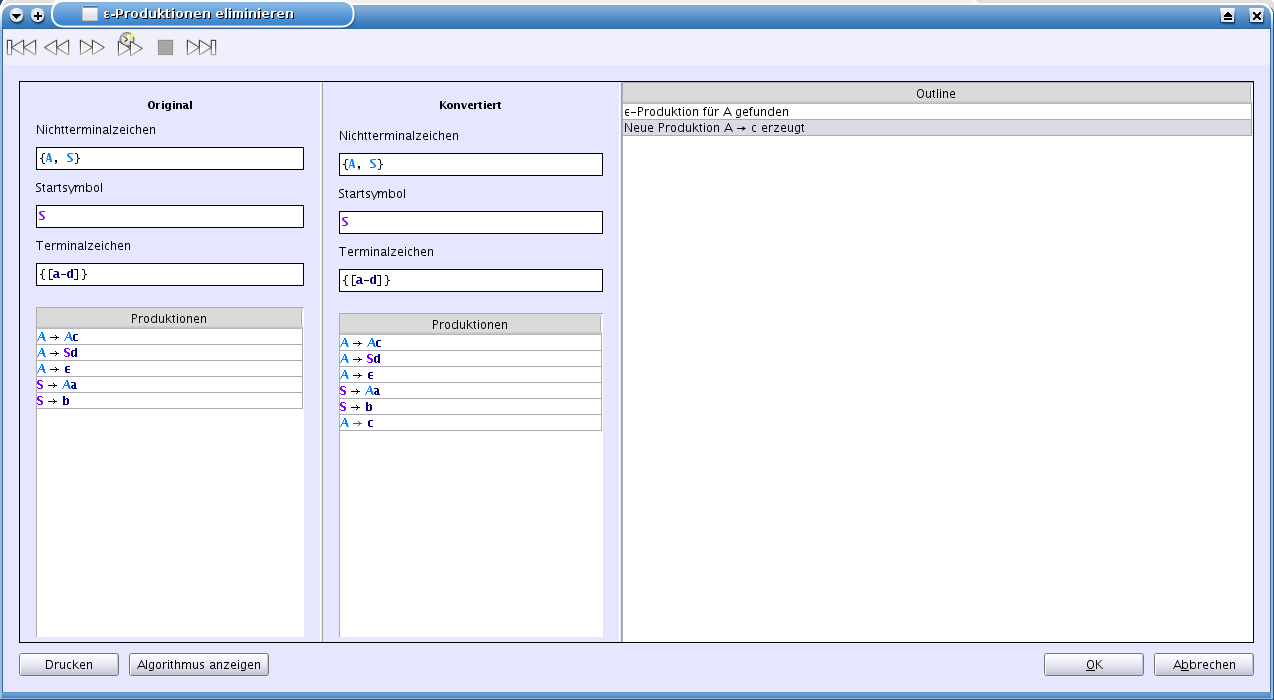
\includegraphics[width=12cm]{../images/epsilon_productions.png}
\caption{Grammatik - $\epsilon$-Produktionen entfernen}
\end{center}
\end{figure}

Dieses Fenster ist im Prinzip das gleiche, wie beim Entfernen der Einheitsproduktionen.

Zunächst sucht der Algorithmus nun nach einer $\epsilon$-Produktion und findet die eine für $\NonterminalSymbol{A}$.

Nun wird für jede Produktion, wo $\NonterminalSymbol{A}$ auf der rechten Seite vorkommt, eine gleiche Produktion, ohne \NonterminalSymbol{A} auf der rechten Seite angelegt. In unserem Beispiel wird zunächst die Produktion $\NonterminalSymbol{A} \to \TerminalSymbol{c}$ und dann $\StartSymbol{S} \to \TerminalSymbol{a}$ angelegt.

Zum Schluss werden die $\epsilon$-Produktionen entfernt, außer der für das Startsymbol. Also in unserem Fall $\NonterminalSymbol{A} \to \epsilon$.


\subsection{Links-Rekursion eliminieren}

Hierzu nutzen wir eine Beispielgrammatik aus der Compilerbau 1-Vorlesung:

\begin{tabular}{lcr}
G = ($\Sigma, N, S, P )\ mit $\\
$\Sigma = \{\TerminalSymbol{a}, \TerminalSymbol{b}, \TerminalSymbol{c},
\TerminalSymbol{d}\}$\\ $N =
\{\NonterminalSymbol{A}, \StartSymbol{S}\}$\\ $S=\StartSymbol{S}$\\
$P = \{\StartSymbol{S} \to \NonterminalSymbol{A}\TerminalSymbol{a},\ \StartSymbol{S} \to \TerminalSymbol{b},\
\NonterminalSymbol{A}	\to \NonterminalSymbol{A}\TerminalSymbol{c},\ \NonterminalSymbol{A} \to \StartSymbol{S}\TerminalSymbol{d},\
\NonterminalSymbol{A} \to \epsilon\}$\\
\end{tabular}

Im Menü findet man unter "`Ausführen"' den Punkt "`Links-Rekursion eliminieren"'. Es erscheint das folgende Fenster.

\begin{figure}[h]
\begin{center}
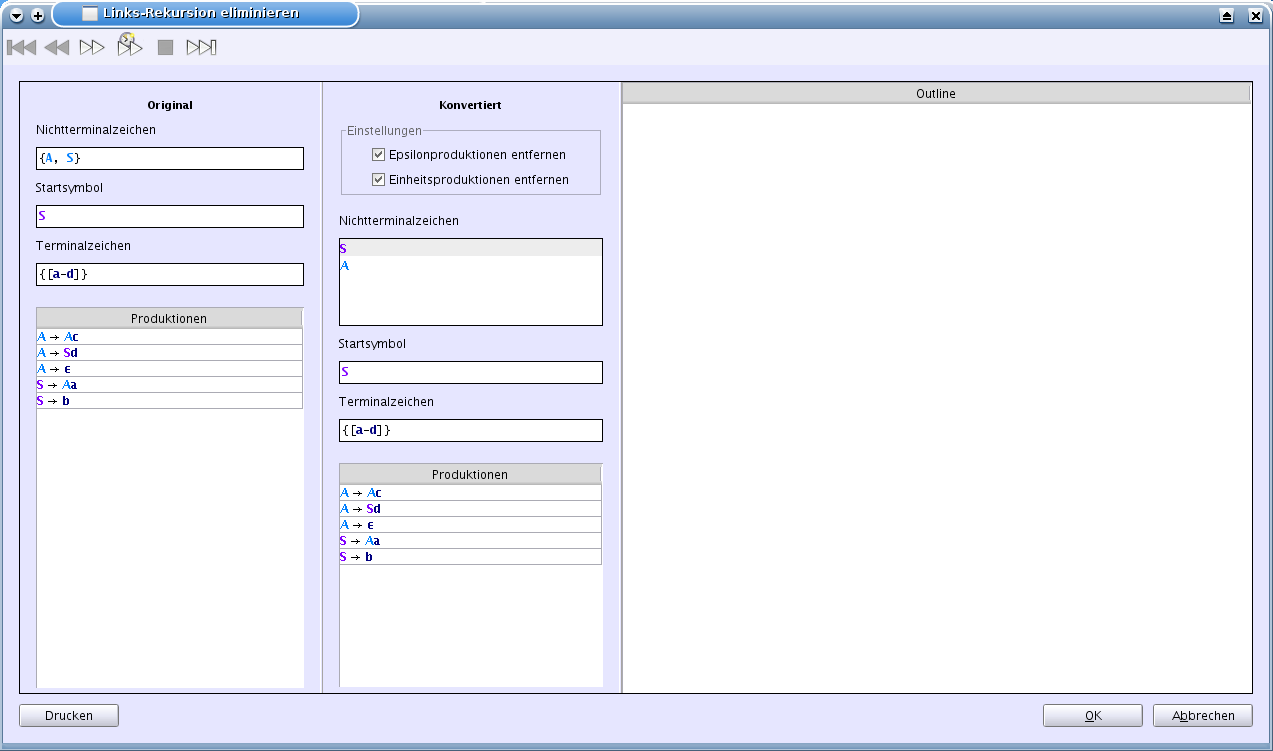
\includegraphics[width=12cm]{../images/left_recursion.png}
\caption{Grammatik - Links-Rekursion eliminieren}
\end{center}
\end{figure}

Dieses Fenster ähnelt den Fenstern zum Entfernen der Einheits- bzw. $\epsilon$-Produktionen.

Oben im Fenster der konvertierten Grammatik kann man einstellen ob zunächst die Epsilon- bzw. Einheitsproduktionen entfernt werden sollen. Diese Möglichkeit wurde gegeben, da der Algorithmus eigentlich eine Grammatik ohne Epsilon- bzw. Einheitsproduktionen verlangt. Aber im Beispiel aus der Vorlesung Compilerbau I wurde die $\epsilon$-Produktion in der Grammatik belassen mit dem Hinweis, dass dies nichts ausmacht. Da aber das Ergebnis dann nicht exakt das selbe wäre, ist hier die Möglichkeit gegeben die Produktionen zu belassen. Für andere Beispiele sollte man aber diese beiden Optionen angestellt lassen, da sonst der Algorithmus falsche Ergebnisse liefern kann.

In unserem Beispiel schalten wir die Option Epsilonproduktionen entfernen aus.

Als nächstes kann die Reihenfolge der Nichtterminalzeichen eingestellt werden, da auch diese sich auf die Ergebnisse des Algorithmus auswirken. Die Reihenfolge kann natürlich genau wie die beiden Optionen zum Entfernen von Produktionen nur am Anfang verändert werden.

In der Vorlesung wurde die Reihenfolge $\StartSymbol{S}, \NonterminalSymbol{A}$ gewählt, daher schieben wir das $\NonterminalSymbol{A}$ einfach nach oben.

Nun kann der Algorithmus ablaufen:

\begin{itemize}
  \item Im initialen Schritt passiert nichts mit der Grammatik, da $i = j$ ist und für $\StartSymbol{S}$ keine direkte Linksrekursion existiert.
  \item Nun kommen durch den Durchlauf im Algorithmus zwei Produktionen ($\NonterminalSymbol{A} \to \NonterminalSymbol{A}\TerminalSymbol{b}\TerminalSymbol{d},\NonterminalSymbol{A} \to \TerminalSymbol{b}\TerminalSymbol{d}$) hinzu und die Produktion $\NonterminalSymbol{A} \to \StartSymbol{S}\TerminalSymbol{d}$ wird entfernt.
  \item Im letzten Schritt dieses Beispiels ist $i = j$ und es wird daher nur noch die direkte Linksrekursion von $\NonterminalSymbol{A}$ entfernt.
\end{itemize}

\subsection{Links-Faktorisierung}

Hierzu nutzen wir folgende Beispielgrammatik aus der Compilerbau 1-Vorlesung:

\begin{tabular}{lcr}
G = ($\Sigma, N, S, P )\ mit $\\
$\Sigma = \{\TerminalSymbol{a}, \TerminalSymbol{b}, \TerminalSymbol{e},
\TerminalSymbol{i},\TerminalSymbol{t}\}$\\ $N =
\{\NonterminalSymbol{E}, \StartSymbol{S}\}$\\ $S=\StartSymbol{S}$\\
$P = \{\StartSymbol{S} \to \TerminalSymbol{i}\NonterminalSymbol{E}\TerminalSymbol{t}\StartSymbol{S}\TerminalSymbol{e}\StartSymbol{S},\StartSymbol{S} \to \TerminalSymbol{i}\NonterminalSymbol{E}\TerminalSymbol{t}\StartSymbol{S}, \StartSymbol{S} \to \TerminalSymbol{a}, \NonterminalSymbol{E} \to \TerminalSymbol{b}$\\
\end{tabular}

Nun findet man im Menü unter "`Ausführen"' den Punkt "`Links-Faktorisierung"'. Es erscheint das folgende Fenster.

\begin{figure}[h]
\begin{center}
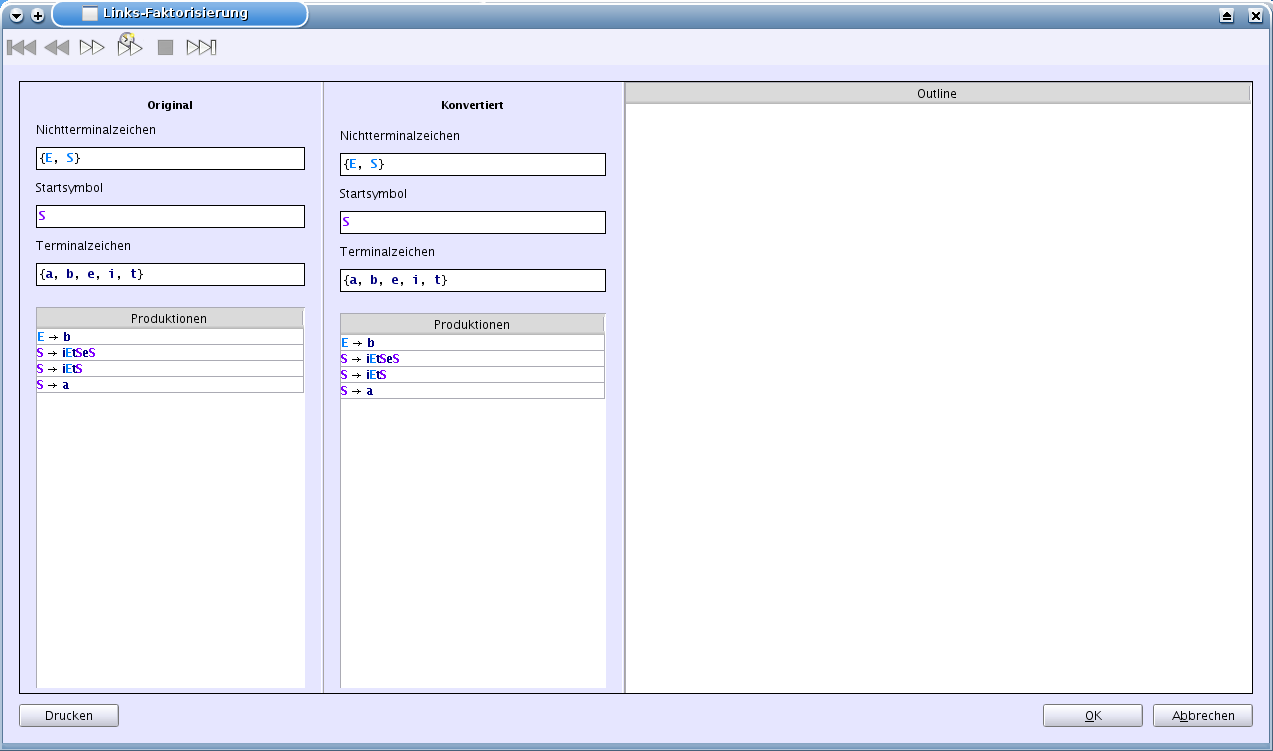
\includegraphics[width=12cm]{../images/left_factoring.png}
\caption{Grammatik - Links-Faktorisierung}
\end{center}
\end{figure}

Ganz links befindet sich die ursprüngliche Grammatik. Rechts daneben findet man die konvertierte Grammatik.

Wenn man den Algorithmus dann ablaufen lässt, ist der Algorithmus bereits nach einem Schritt fertig. Der Algorithmus findet als längstes gemeinsames Präfix $\TerminalSymbol{i}\NonterminalSymbol{E}\TerminalSymbol{t}\StartSymbol{S}$ und erzeugt ein neues Nichtterminalzeichen $\NonterminalSymbol{S'}$. Als Produktionen kommen hinzu: $\StartSymbol{S} \to \TerminalSymbol{i}\NonterminalSymbol{E}\TerminalSymbol{t}\StartSymbol{S}\NonterminalSymbol{S'}, \NonterminalSymbol{S'} \to \epsilon, \NonterminalSymbol{S'} \to \TerminalSymbol{e}\StartSymbol{S}$, entfernt wurde die Produktion $\StartSymbol{S} \to \TerminalSymbol{i}\NonterminalSymbol{E}\TerminalSymbol{t}\StartSymbol{S}\TerminalSymbol{e}\StartSymbol{S}$.

\subsection{Recursive Descent Parser erstellen}

Hierzu nutzen wir eine Beispielgrammatik aus der Compilerbau 1-Vorlesung:

\begin{tabular}{lcr}
G = ($\Sigma, N, S, P )\ mit $\\
$\Sigma = \{\TerminalSymbol{a}, \TerminalSymbol{b}, \TerminalSymbol{e},
\TerminalSymbol{i},\TerminalSymbol{t}\}$\\ $N =
\{\NonterminalSymbol{E}, \StartSymbol{S}\}$\\ $S=\StartSymbol{S}$\\
$P = \{\StartSymbol{S} \to \TerminalSymbol{i}\NonterminalSymbol{E}\TerminalSymbol{t}\StartSymbol{S}\TerminalSymbol{e}\StartSymbol{S},\StartSymbol{S} \to \TerminalSymbol{i}\NonterminalSymbol{E}\TerminalSymbol{t}\StartSymbol{S}, \StartSymbol{S} \to \TerminalSymbol{a}, \NonterminalSymbol{E} \to \TerminalSymbol{b}$\\
\end{tabular}

Nun findet man im Menü unter "`Ausführen"' den Punkt "`Recursive Descent Parser erstellen"'. Es erscheint das folgende Fenster.

\begin{figure}[h]
\begin{center}
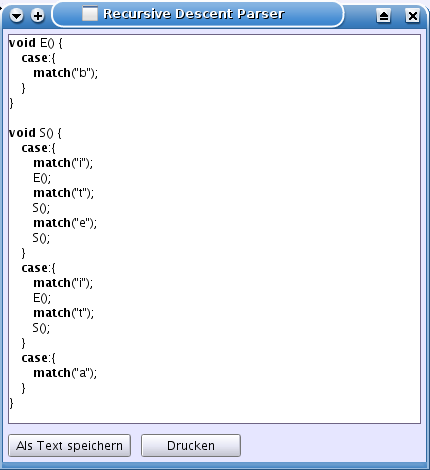
\includegraphics[width=6cm]{../images/rdp.png}
\caption{Grammatik - Recursive Descent Parser}
\end{center}
\end{figure}

Es wurde der Recursive Descent Parser in einer einfachen Programmiersprache erstellt.

Es wird für jedes Nonterminal eine Funktion erstellt. Also in unserem Beispiel zunächst eine für \NonterminalSymbol{E}. Darin werden dann verschiedene Fälle behandelt. Da es für \NonterminalSymbol{E} nur die Produktion $\NonterminalSymbol{E} \to \TerminalSymbol{b}$ gibt, gibt es auch nur einen Fall. In diesem wird das Eingabezeichen \TerminalSymbol{b} gelesen, angedeutet durch das macht("b").

Danach wird eine Funktion für \NonterminalSymbol{S} erstellt. Diese beinhaltet drei Fälle. Zunächst wird im ersten Fall die erste Produktion von \NonterminalSymbol{S} behandelt. Als erstes wird \TerminalSymbol{i} gelesen, dann wird die Funktion für das Nonterminal \NonterminalSymbol{E} aufgerufen und so weiter.

Den Recursive Descent Parser kann man entweder als Text speichern oder drucken.

\subsection{Deterministischer Recursive Descent Parser erstellen}

Um den DRDP zu erstellen geht man analog der Erstellung des RDP vor, wie im vorhergehenden Abschnitt beschrieben. Sollte die Grammatik nicht in LL1 liegen, so wird
eine Fehlermeldung angezeigt:

\begin{figure}[h]
  \begin{center}
    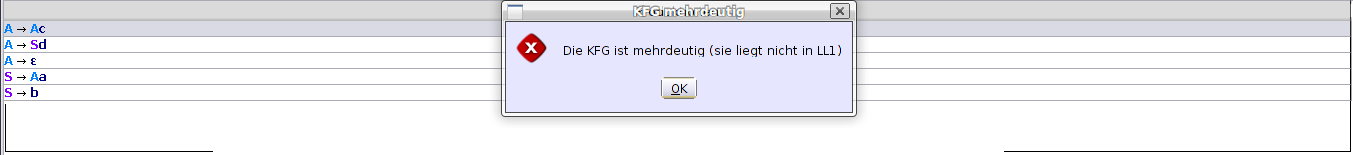
\includegraphics[scale=0.25]{../images/cfgnotll1.png}
    \caption{Grammatik liegt nicht in LL1}
  \end{center}
\end{figure}

\newpage
Wenn die Grammatik in LL1 liegt, so wird der deterministische Recursive Descent Parser erzeugt:

\begin{figure}[h]
  \begin{center}
    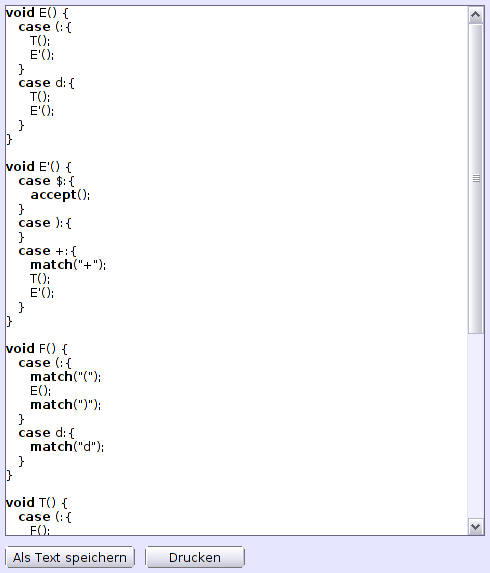
\includegraphics[width=6cm]{../images/deterministicrdp.png}
    \caption{Deterministischer Recursive Descent Parser}
  \end{center}
\end{figure}



%%
%% $Id$
%%
%% Copyright (c) 2007-2008 Christian Fehler
%% Copyright (c) 2007-2008 Benjamin Mies
%%


\chapter{Umwandeln}\label{ConverTo}

In diesem Kapitel soll das Umwandeln von einer Grammatik in einen Automaten
bzw. zwischen den verschiedenen Automaten Typen besprochen werden. Dabei wird
im Besonderen darauf eingegangen, welche Herausforderungen aufgetreten sind, um
dem Benutzer die verwendeten Algorithmen möglichst in kleinen Schritten und
verständlich darzustellen. Beim Umwandeln der Grammatiken in die entsprechenden
Automaten sind die verwendeten Algorithmen leicht zu verstehen und zusätzlich
nicht besonders gut darzustellen, weshalb hier darauf verzichtet wurde, dem
Benutzer eine schrittweise Umwandlung anhand einer graphischen Darstellung zu
präsentieren.\vspace{10pt}


\section{Grammatik umwandeln}\label{ConverToGrammar}

Wenn ein Benutzer eine Grammatik vollständig erstellt hat, kann es durchaus
interessant sein, den Automaten zu sehen, welcher die Sprache akzeptiert, die
durch die Grammatik beschrieben wird. Vor allem, da für Automaten weitaus mehr
Verwendungsmöglichkeiten in diesem Werkzeug existieren.\vspace{10pt}

\subsection{Umwandeln einer regulären Grammatik}\label{ConverToGrammarRegular}

Eine reguläre Grammatik kann in einen entsprechenden nicht deterministischen
endlichen Automaten umgewandelt werden. Die Zustände unseres entstehenden
Automaten resultieren aus den Nichtterminalzeichen unserer Grammatik. Allerdings
werden in der Implementierung nur Zustände für die Nichtterminalzeichen angelegt,
welche auch in einer Produktion, auf der rechten oder linken Seite, verwendet
werden. Die Zustände werden immer dann angelegt, wenn man auf ein
Nichtterminalzeichen trifft, welches man bis jetzt noch nicht gesehen
hat.\vspace{10pt}

Die Rechte Seite einer Produktion kann entweder aus einem einzelnen
Terminalzeichen bestehen ($\NonterminalSymbol{S} \to \TerminalSymbol{a}$), oder
aus einem Terminalzeichen mit einem anschließenden Nichtterminalzeichen
($\NonterminalSymbol{S} \to \TerminalSymbol{a}\NonterminalSymbol{A}$). Da keine
anderen Produktionen für diese Grammatikform existieren können.\vspace{10pt}

Wir schauen uns jetzt jede Produktion unserer Grammatik an.
Zunächst interessiert uns die linke Seite. Wenn wir das Nichtterminalzeichen
bereits gesehen haben, wurde auch schon ein Zustand dafür angelegt, und wir
merken uns diesen. Wenn wir das Nichtterminalzeichen noch nicht gesehen haben,
müssen wir jetzt einen neuen Zustand anlegen, welcher dieses repräsentiert, und
merken uns diesen neuen Zustand, da dieser der Ausgangszustand
für neu enstehende Übergänge ist.\vspace{10pt}

Als nächstes betrachten wir die rechte Seite der Produktion. Wenn es sich dabei
um ein einzelnes Terminalzeichen handelt, wird ein neuer akzeptierender Zustand
angelegt. Danach wird ein Übergang von dem Zustand für das Nichtterminalzeichen
zu diesem neuen Zustand erzeugt, wobei die Übergangsmenge aus dem
Terminalzeichen auf der rechten Seite der Produktion besteht.\vspace{10pt}

Besteht die rechte Seite allerdings aus einem Terminalzeichen und einem
Nichtterminalzeichen müssen wir wieder überprüfen, ob wir das
Nichtterminalzeichen bereits gesehen haben, um gegebenenfalls den
entsprechenden Zustand anzulegen. Im nächsten Schritt wird ein Übergang,
zwischen den beiden Zuständen die wir uns gemerkt haben, angelegt, mit dem
Terminalzeichen der rechten Seite als Übergangsmenge.\vspace{10pt}

Diese Behandlung wiederholen wir für jede Produktion unserer Grammatik und
erhalten so den entsprechenden Automaten.\vspace{10pt}

\subsection{Umwandeln einer kontextfreien Grammatik}\label{ConverToGrammarContextFree}

Der Benutzer hat auch die Möglichkeit, eine konstruierte kontextfreie Grammatik
in einen Kellerautomaten umwandeln zu lassen.\vspace{10pt}

Bei diesem Algorithmus werden zwei Zustände angelegt. Ein Startzustand und ein
akzeptierender Zustand. Dazu ein Übergang vom Startzustand in den
akzeptierenden Zustand, welcher das Startsymbol der Grammatik in den Keller
legt. Dann wird für jede Produktion ein Übergang angelegt, welcher die rechte
Seite der Produktion vom Keller entfernt, und dafür die linke Seite der
Produktion auf den Keller schreibt. Dieser Übergang hat als
Ursprungs- und Zielzustand den akzeptierenden Zustand.\vspace{10pt}

Wenn alle Produktion verarbeitet wurden, werden noch zusätzlich pro
Terminalzeichen ein Übergang angelegt. In jedem dieser Übergänge wird das
entsprechende Terminalzeichen vom Eingabewort gelesen und vom Keller des
Automaten genommen. Das bedeutet, es muss das gleiche Terminalzeichen als
oberstes im Keller  und als nächstes Zeichen im Wort stehen.\vspace{10pt}

Durch die Zweite Ansicht (siehe Kapitel \ref{SecondView}) hat der Benuzter auch
die Möglichkeit die Ausgangsgrammatik und den enstandenen Automaten nebeneinander
zu sehen, um die Zusammenhänge besser verstehen zu können.\vspace{10pt}


\section{Automat umwandeln}\label{ConverToMachine}

Bei der Planung der Umwandlung zwischen den verschiedenen Automaten Typen
stellte sich die Frage, wie dem Benutzer der Umwandlungsalgorithmus möglichst
verständlich dargestellt wird. Wir entschieden uns für das auch sonst im
\gtitool verwendete Verfahren, eine Navigationsleiste zu verwendet, die es dem
Benutzer gestattet in dem Algorithmus einen Schritt vor, bzw. einen Schritt
zurück zu gehen. Um die Handhabung für den Benutzer zu erleichtern, wurde die
Navigationsleiste so erweitert, dass der Benutzer zurück an den Anfang der
Ausführung des Algorithmus springen kann, ebenfalls an das Ende und, dass die
einzelnen Schritte auch automatisch, nach einer einstellbaren Zeit, durchgeführt
werden können.\vspace{10pt}

Um dem Benutzer den durchgeführten Algorithmus zu verdeutlichen, wurde die
Ansicht in drei Bereiche eingeteilt. In dem oberen linken Bereich wird der
Ausgangsautomat dargestellt, im unteren linken Bereich der nach und nach
endstehende konvertierte Automat und schließlich im rechten Bereich eine
Outline, die pro Schritt, jeweils mit einem Kommentar, angibt, welchen Schritt
der Algorithmus im Moment durchführt.\vspace{10pt}

\begin{figure}[h!]
\begin{center}
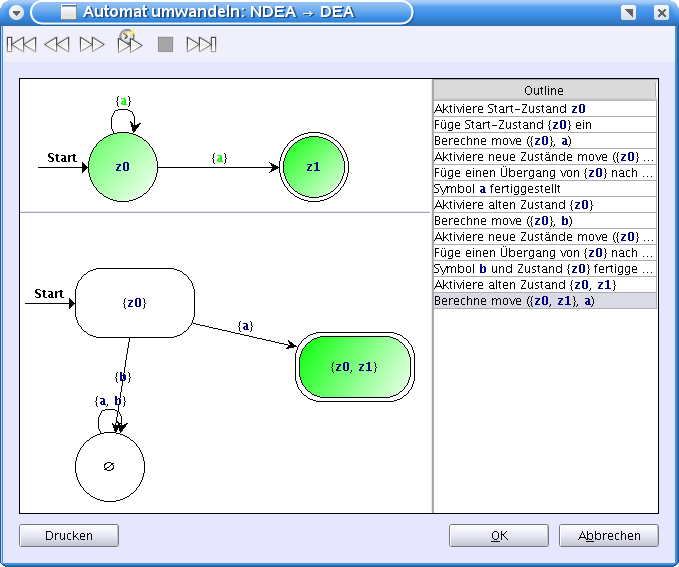
\includegraphics[width=12cm]{../images/convert_to.png}
\caption{Automat umwandeln}
\end{center}
\end{figure}
\vspace{10pt}

Es existieren zwei verschiedene Verfahren zur Umwandlung in einen
deterministischen endlichen Automaten (DEA). Zum einen kann der komplette
Potenzautomat verwendet werden, um den DEA zu erzeugen. Der entstehende Automat
enthält allerdings unter Umständen sehr viele nicht erreichbare Zustände, deren
Berechnung einige zusätzliche Schritte zur Folge haben kann. Wenn der Benutzer
diese Art der Umwandlung auswählt, kann er nach dem Umwandeln die nicht
erreichbaren Zustände wieder entfernen, wie dies funktioniert, kann in
\ref{ReachableStates} nachgelesen werden. Die zweite Methode ist, dass nur die
erreichbaren Zustände in der unteren Ansicht angelegt werden. Diese Methode ist
übersichtlicher für den Benutzer, wenn auch nicht alle im Potenzautomaten
vorhandenen Zustände betrachtet werden.\vspace{10pt}

\newpage
%### removes texlipse warning
Zur Umsetzung wurde der in \cite[S. 153ff]{Compilers} angegebene Algorithmus als
Vorlage benutzt. Um den Algorithmus verwenden zu können, müssen zuerst einige
Werte definiert werden.\vspace{10pt}
%### removes texlipse warning

\noindent
\begin{tabular}{|p{2.2cm}|p{9.0cm}|}
  \hline
  NFA A                 & Input NFA \\
  \hline
  DFA D                 & Output DFA \\
  \hline
  Dstates               & States of output DFA D \\
  \hline
  Dtran                 & Transition function of DFA D \\
  \hline
  $\epsilon$-closure(s) & Set of NFA states reachable from NFA state s
                          on $\epsilon$-transitions alone \\
  \hline
  $\epsilon$-closure(T) & Set of NFA states reachable from some NFA state s
                          in set T on $\epsilon$-transitions alone; =
                          $\cup_{s\ in\ T}\ \epsilon$-closure(s). \\
  \hline
  move(T,a)             & Set of NFA states to which there is a transition
                          on input symbol a from some state s in T \\
  \hline
\end{tabular}
\vspace{10pt}

Die eigentliche Umwandlung geschieht dann mit folgendem Algorithmus, der aus
didaktischen Gründen in mehrere Schritte aufgeteilt wurde.\vspace{10pt}

\noindent
\verb| 1 initially, |$\epsilon$\verb|-closure(|$s_0$\verb|) is the only state in Dstates,|\\
\verb| 2 and it is unmarked;|\\
\verb| 3 while ( there is an unmarked state T in Dstates ) {|\\
\verb| 4       mark T;|\\
\verb| 5       for ( each input symbol a ) {|\\
\verb| 6           U = |$\epsilon$\verb|-closure(move(T,a));|\\
\verb| 7           if ( U is not in Dstates )|\\
\verb| 8              add U as an unmarked state to Dstates;|\\
\verb| 9           Dtran[T,a] = U;|\\
\verb|10       }|\\
\verb|11 }|
\vspace{10pt}


%%
%% $Id$
%%
%% Copyright (c) 2007-2008 Christian Fehler
%% Copyright (c) 2007-2008 Benjamin Mies
%%


\chapter{Minimieren}\label{Minimize}

Wenn wir einen Automaten erstellt haben können wir mit diesem schon alle
Funktionen, welche dieses Lernwerkzeug bietet, nutzen. Allerdings besteht die
Möglichkeit, dass ein Automat existiert, der die gleiche Sprache erkennt die
unser erstellter Automat erkennt, jedoch mit weniger Zuständen auskommt. Bei
komplexeren Beispielen bemerkt man schnell, dass die Übersichtlichkeit mit
wachsender Anzahl der Zustände immer weiter abnimmt. Daher ist es wünschenswert
immer mit dem minimalen Automaten für eine bestimmte Sprache zu arbeiten. Im
folgenden wollen wir uns jetzt den Algorithmus ansehen, welcher verwendet wird,
um aus einem Automaten einen neuen Automaten mit einer minimalen Anzahl von
Zuständen zu erzeugen.\vspace{10pt}

Wie bereits erwähnt erhält der Algorithmus als Eingabe einen Automaten, und als
Ausgabe erwarten wir einen Automaten der die gleiche Sprache akzeptiert wie
unser Eingabeautomat, jedoch mit so wenig wie möglich Zuständen
auskommt.\vspace{10pt}

Unser erster Minimierungsschritt besteht darin, die Zustände zu entfernen, die
ausgehend vom Startzustand nicht erreichbar sind. Denn wenn die Zustände nicht
erreicht werden, können sie auch keine Auswirkung auf die Sprache haben, welche
der Automat erkennt.\vspace{10pt}

Im weiteren versuchen wir äquivalente Zustände in Gruppen, auch
Äquivalenz\-klassen genannt, zusammenzufassen, um diese später zu einem Zustand
zu verschmelzen. Initial wird unsere Menge von Zuständen in zwei Gruppen
unterteilt. Alle akzeptierenden Zustände bilden die erste Gruppe, und die
zweite Gruppe besteht aus allen nicht akzeptierenden Zuständen.\vspace{10pt}

Wir nehmen uns jetzt das Alphabet unseres Eingabeautomaten zur Hilfe um zu
prüfen, ob alle Zustände einer Gruppe wirklich in einer Äquivalenzklasse
liegen, oder ob wir die Gruppe aufspalten können. Dazu sei gesagt, dass zwei
Zustände in der selben Äquivalenzklasse ligen, wenn sie mit jeweils allen
Symbolen des aktuellen Alphabets in einen Zustand der selben Gruppe
übergehen.\vspace{10pt}

  \begin{figure}[h]
  \begin{center}
  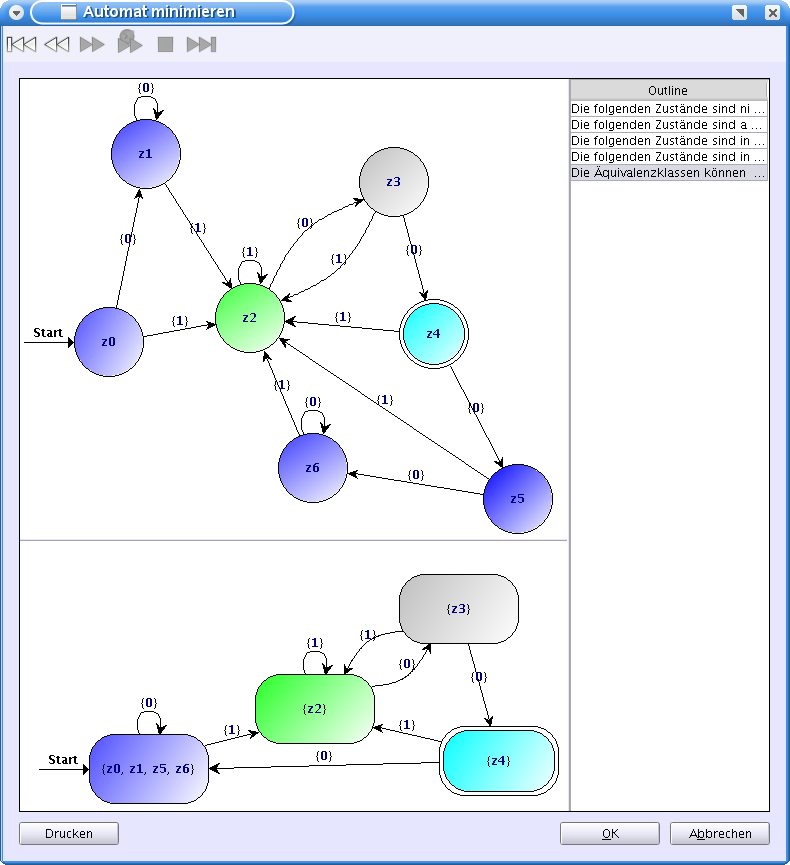
\includegraphics[width=12cm]{../images/minimize.png}
  \caption{Automat - Minimieren}
  \end{center}
  \end{figure}

Schauen wir uns jetzt mal die Arbeitsweise des Algorithmus im Detail an. Als
erstes müssen wir uns die aktuelle Gruppeneinteilung merken, also wieviele
Gruppen wir haben, und welcher Zustand in welcher Gruppe liegt. Wir betrachten
die erste unserer Gruppen. Wenn diese nur einen Zustand enthält kann sie nicht
weiter verfeinert werden, und muss daher auch nicht mehr betrachtet werden.
\vspace{10pt}

Wenn die Gruppe mehr als einen Zustand beinhaltet, nehmen wir uns das aktuelle
Alphabet des Automaten zur Hilfe. Wir prüfen jetzt für jedes Symbol des Alphabets
einzeln, ob alle Zustände der Gruppe mit diesem Symbol in Zustände der selben
Gruppe übergehen. Wenn das der Fall ist kann auch diese Gruppe nicht weiter
unterteilt werden. Falls wir aber doch auf Zustände treffen, welche in eine
andere Gruppe übergehen, werden diese Zustände aus der aktuellen Gruppe entfernt,
und bilden eine neue Gruppe. \vspace{10pt}

Nachdem wir diese Prozedur für diese Gruppe
abgeschlossen haben, wiederholen wir sie für alle Gruppen die wir noch nicht
betrachtet haben. Nach Betrachtung aller Gruppen vergleichen wir die aktuelle
Gruppeneinteilung mit der, die wir uns gemerkt haben. Wenn diese übereinstimmt,
ist unser Algorithmus am Ende, und die Gruppen können nicht weiter verfeinert
werden. Stimmt die Gruppeneinteilung nicht überein, müssen wir wieder jede
Gruppe einzeln betrachten, und versuchen diese in kleiner Gruppen zu
zerlegen.\vspace{10pt}

Nach Beendigung des Algorithmus repräsentiert jede Gruppe einen Zustand
in unserem neuen Automaten. Jetzt muss noch pro Symbol des Alphabets der
Übergang in den entsprechenden neuen Zustand angelegt werden. Mit diesem
letzten Schritt ist die Konstruktion des minimalen Automaten
abgeschlossen.\vspace{10pt}

In unserem Lernwerkzeug wird dem Benutzer in einer sogenannten Outline genau
mitgeteilt, was in den bisherigen Schritten des Algorithmus passiert ist.
Desweiteren ermöglichen wir dem Benutzer eine schrittweise Navigation und Vor-
und Rückrichtung. Diese beiden Features sollen es ermöglichen den
Minimierungsalgorithmus besser nachvollziehen und verstehen zu
können.\vspace{10pt}




%%
%% $Id$
%%
%% Copyright (c) 2007-2008 Christian Fehler
%% Copyright (c) 2007-2008 Benjamin Mies
%%


\chapter{Auto Layout}\label{AutoLayout}

Beim Anlegen eines neuen Automaten, oder auch modifizieren eines bestehenden,
kommt es vor, dass die Übersichtlichkeit verloren geht. Damit man eine schnelle
Möglichkeit hat, den Automaten wieder besser überblicken zu können wurde eine
Autolayout Funktion implementiert.\vspace{10pt}

Diese Funktion basiert zur Zeit auf dem Erweiterten Partitionierungsalgorithmus
von Kerninghan und Lin , welcher auch als "`Min Cut"'- Algorithmus
bekannt ist. Er beruht auf iterativer Verbesserung durch paarweisen
Austausch.\vspace{10pt}

Dieser Algorithmus wird eigentlich für die Partitionierung von Schaltungen
verwendet, kann aber problemlos auf unsere Situation übertragen werden.
Allerdings mussten bei der Übertragung einige Modifikationen
vorgenmommen werden, auf welche ich später noch näher eingehen
möchte.\vspace{10pt}

\section{Der Kerninghan-Lin-Algorithmus im Details}

Zu Beginn wird das Partitionierungsproblem in eine Graphendarstellung
transformiert. Danach werden die Knoten des Graphen in zwei Gruppen unterteilt.
Anschließend werden für die aktuelle Einteilung die Schnittkosten berechnet.
Zur Berechnung der Schnittkosten werden die von der Schnittlinie, die Linie die
die beiden Gruppen trennt, erfassten Kanten gezählt.\vspace{10pt}

%### removes texlipse warning
Der Kerninghan-Lin-Algorithmus lässt sich in die folgenden Schritte
unterteilen, welche dem Buch "`Layoutsynthese elektronischer
Schaltungen"' (\cite{Layout}) entnommen wurden:\vspace{10pt}
%### removes texlipse warning

Schritt 0:
\begin{itemize}
  \item V = Menge der 2n Knoten 
  \item {A,B} sei eine willkürliche Anfangspartitionierung
\end{itemize}

Schritt 1:
\begin{itemize}
  \item i=1
  \item Berechnung von D(v) für alle Knoten v $\in$ V
\end{itemize}

Schritt 2:
\begin{itemize}
  \item Auswahl von $a_i$ und $b_i$ mit maximalem Gewinnwert $\Delta g_i =
  D(a_i) + D(b_i) - 2 * c(a_i b_i)$
  \item Vertauschen und fixieren von $a_i$ und $b_i$
\end{itemize}


Schritt 3:
\begin{itemize}
  \item Wenn alle Knoten fixiert sind, weiter mit Schritt 4, andernfalls
  \item Neuberechnung der D-Werte für alle Knoten, welche nicht fixiert und
  mit $a_i$ und $b_i$ verunden sind
  \item i=i+1
  \item Weiter mit Schritt 2
\end{itemize}

Schritt 4:
\begin{itemize}
  \item Bestimmung der Vertauschungssequenz 1 bis m $(1 \leq m \leq i)$, so dass
  $G_m = \sum_{i=1}^{m}{\Delta g_i}$ maximiert wird
  \item Wenn $G_m > 0$, weiter mit Schritt 5, andernfalls ENDE
\end{itemize}

Schritt 5:
\begin{itemize}
  \item Durchführen alle m Vertauschungen, Beseitigen aller Knotenfixierungen
  \item Weiter mit Schritt 1
\end{itemize}\vspace{10pt}

Schauen wir uns zunächst einmal an, wie der Algorithmus vorgeht, indem wir
nachvollziehen, was in den einzelnen Schritten passiert.\vspace{10pt}

In $Schritt\ 0$ werden die Knoten in zwei gleichgroße Gruppen unterteilt, wobei
es keine Rolle spielt, welcher Knoten in welcher Gruppe landet. Danach werden in
$Schritt\ 1$ für alle Knoten berechnet, ob sie einen hohen oder niedrigen Anteil
der Schnittkosten verursachen. Der Gewinnwert $\Delta g$, welcher in $Schritt\
2$ erwähnt wird, beschreibt die Verbesserung der Schnittkosten, welche durch
einen Knotentausch erreicht werden kann. Die beiden Knoten, welche den
maximalen Gewinnwert bringen, werden dann getauscht und fixiert. In $Schritt\ 3$
überprüfen wir ob alle Knoten bereits fixiert sind, ansonsten werden die Kosten
für jeden Knoten der noch nicht fixiert ist neu berechnet und erneut $Schritt\
2$ ausgeführt. In $Schritt\ 4$ wird überprüft ob der Algorithmus bereits sein
Ende erreicht hat. Wenn nicht, werden in $Schritt\ 5$ die Vertauschungen des
aktuellen Durchgangs durchgeführt, und es wird ein neuer Durchgang gestartet.\vspace{10pt}

%### removes texlipse warning
Wie schon erwähnt musste der Algorithmus für die Implementierung ein wenig
modifiziert werden. Zum einen  geht man eigentlich davon aus, dass die Knoten
in zwei etwa gleichgroße Gruppen einteilt. Dies erwies sich bei der
Implementierung allerdings als eher unvorteilhaft. Daher wird dynamisch
bestimmt, in wieviele Gruppen die Knoten unterteilt werden, wobei die Größe
aller Gruppen aber auch hier in etwa die gleiche ist. Diese
Implementierung entspricht soweit der Erweiterung des
Kerningham-Lin-Algorithmus wie sie in \cite{Layout} beschrieben
wird\vspace{10pt}
%### removes texlipse warning

Die Erweiterung des Algorithmus sieht jetzt vor, dass man den Algorithmus jetzt
für alle möglichen zweier Paarungen von Gruppen betrachtet. Die Implementierung
sieht so aus, dass man eine Linie zwischen die erste und zweite Gruppe legt,
und jetzt alle Kanten zählt, die diese Linie schneiden. Jetzt wird berechnet, bei welchen
beiden Knoten ein Tausch die größte Verbesserung liefert, also die meißten
Schnitte mit der Linie wegfallen. Diese werden dann getauscht und fixiert. Wenn
alle Knoten fixiert sind, oder keine Tauschkombination existiert bei der
Schnitte mit der Linie zwischen den Gruppen wegfallen, wird die Linie eine
Gruppe nach unten geschoben, also zwischen die zweite und dritte Gruppe und die
Vorgehensweise wiederholt. Der Algorithmus terminiert, nachdem die vorletzte und
letzte Gruppe abgearbeitet wurden.\vspace{10pt}

Dieser Algorithmus liefert noch nicht das optimale Ergebnis, was zum Beispiel
auch daran liegt, dass die Länge der Kanten in keinster Weise berücksichtigt
werden. Daher wird im Kapitel \ref{PerspectiveAutoLayout} ein alternativer
Algorithmus beschrieben, welcher wahrscheinlich bessere Ergebnisse für ein
automatischen Layout liefern könnte.


%%
%% $Id$
%%
%% Copyright (c) 2007-2008 Christian Fehler
%% Copyright (c) 2007-2008 Benjamin Mies
%%


\chapter{Interaktion}\label{Interaction}

In diesem Kapitel werden die Interaktionen mit dem Benutzer erläutert. Ein
wichtiger Aspekt der Interaktionen ist, dass der Benutzer angezeigt bekommt,
wenn er etwas falsches eingeben hat. Ein weiterer Punkt ist, dass der Benutzer
bei einem nicht deterministischen Kellerautomaten auswählen muss, welchen
Übergang der Automat machen soll, da dieser das im Allgemeinen nicht erkennen
kann.\vspace{10pt}


\section{Fehler und Warnung}\label{InteractionErrorWarning}

Es war uns bei der Umsetzung des \gtitools sehr wichtig, dass der Benutzer sehr
viele Fehler machen kann, ohne dass er durch eine Validierung eingeschränkt wird.
Eine Ausnahme von diesem Konzept bilden die in Kapitel \ref{Parser} beschriebenen
Parser, da eine falsche Eingabe dort nicht anständig durch das Anzeigen von
Fehlern bzw. Warnungen behandelt hätte werden können.\vspace{10pt}

Der Hauptgrund für die Auswahl dieser Strategie war, dass der Benutzer durch das
fehlerhafte Eingeben bzw. durch das Beheben der Fehler hoffentlich mehr lernt,
als wenn er die Eingaben gar nicht erst hätte machen können. In diesem Abschnitt
werden die verschiedenen Fehler und Warnungen beschrieben, die bei Grammatiken und
Automaten auftreten können.\vspace{10pt}


\subsection{Grammatik}

Im Folgenden möchten wir auf die Fehler und Warnungen eingehen, welche bei dem
Validierungsvorgang einer Grammatik auftreten können.\vspace{10pt}

Als Validierungsfehler zählt, unter anderem, wenn die gleiche Produktion mehrfach
angelegt wurde. In der Spalte Meldung sieht man wie immer nur, um welchen Fehler
es sich gerade handelt. Über die Beschreibung wird mitgeteilt, um welche
Produktion es sich dabei handelt. Man kann sich die betreffenden Produktionen
auch farblich hervorheben lassen, indem man die entsprechende Fehlermeldung durch
Mausklick auswählt. So kann der Benutzer die fehlerhaften Produktionen schnell
lokalisieren und den Fehler beheben.\vspace{10pt}

Wenn es sich bei der aktuellen Grammatik um eine reguläre Grammatik handelt,
gibt es noch eine weitere Fehlermeldung. Wenn nicht alle Produktion dem
vorgegebenen Muster für eine rechtsreguläre Grammtik entsprechen, wird dies auch
über einen Validierungsfehler angezeigt. Dabei kann man auch hier anhand der
Beschreibung sehen, um welche Produktion es sich handelt. Wenn man den
entsprechenden Eintrag auswählt, wird dem Benutzer wieder durch farbiges
Hervorheben signalisiert, wo sich diese Produktion befindet. Es wird jetzt
allerdings nicht die komplette Produktion eingefärbt, sondern nur der Teil der
Satzform, welcher nicht dem Muster entspricht. Auch hier war wieder die
Intention, dem Benutzer schnell zu einer gültigen Grammatik zu
verhelfen.\vspace{10pt}

Neben diesen beiden Fehlern haben wir auch eine Warnung eingeführt. Diese gibt
Auskunft darüber, wenn ein Nichtterminalzeichen, vom Startsymbol ausgehend,
nicht ableitbar ist. Es handelt sich hierbei nur um eine Warnung, weil es sich
durchaus um eine gültige Grammatik handeln kann. Sie soll dem Benutzer allerdings
dazu animieren, die Übergangsmenge zu kontrollieren, ob nicht eine, oder mehrere
Produktionen vergessen wurden. So soll es möglich sein, Flüchtig\-keits\-fehler
frühzeitig zu erkennen und zu beheben.\vspace{10pt}

\subsection{Automat}

Auch für den Automaten gibt es einige Fehler und Warnungen die nun aufgezählt
werden. Die verschiedenen Automatentypen verwenden unterschiedliche Fehler. So
ist ein $\epsilon$-Übergang in einem $\epsilon$-NDEA kein Fehler, in einem DEA
aber schon. Deshalb wird bei jedem Fehler angegeben, in welchem Automaten er
vorhanden ist.\vspace{10pt}

\noindent
\begin{tabular}{|p{2.1cm}|p{2.7cm}|p{6.0cm}|}
  \hline
  Alle Symbole &
  DEA &
  Ein Zustand muss Übergänge mit allen Symbolen enthalten \\
  \hline
  Symbole nur einmal &
  DEA und Kellerautomat &
  Ein Zustand darf nicht mehrere Übergänge mit dem gleichen Symbol enthalten \\
  \hline
  $\epsilon$-Übergang &
  DEA und NDEA &
  Es darf kein $\epsilon$-Übergang vorhanden sein \\
  \hline
  Keller-Operationen &
  DEA, NDEA und $\epsilon$-NDEA &
  Es dürfen keine Operationen auf dem Keller ausgeführt werden \\
  \hline
  Mehr als ein Start-Zustand &
  DEA, NDEA, $\epsilon$-NDEA und Kellerautomat&
  Es darf nur ein Start-Zustand vorhanden sein \\
  \hline
  Kein Start-Zustand &
  DEA, NDEA, $\epsilon$-NDEA und Kellerautomat&
  Es muss ein Start-Zustand vorhanden sein \\
  \hline
  Eindeutiger Zustandsname &
  DEA, NDEA, $\epsilon$-NDEA und Kellerautomat&
  Die Namen der Zustände müssen eindeutig sein \\
  \hline
\end{tabular}
\vspace{10pt}

\noindent
Neben diesen Fehlern gibt es auch noch zwei Warnungen. Zum einen wird der
Benutzer gewarnt, wenn kein akzeptierenden Zustand vorhanden ist. Dabei handelt
es sich nicht um einen ungültigen Automaten, aber es könnte sein, dass der
ungeübte Benutzer den akzeptierenden Zustand nur vergessen hat. Außerdem wird
eine Warnung angezeigt, wenn ein oder mehrere Zustände nicht erreichbar sind.
Zur Bestimmung dieser unerreichbaren Zustände wird der gleiche Algorithmus
verwendet, der auch bei den erreichbaren Zuständen in Kapitel
\ref{ReachableStates} benutzt wird.\vspace{10pt}


\section{Operationen mit dem Automaten Keller}\label{InteractionPDA}

Ein wichtiger Punkt der Interaktion mit dem Benutzer ist, dass der Benutzer
nach einer Umwandlung einer kontextfreien Grammatik in einen Kellerautomaten
einen Übergang auswählen muss, weil der entstehende Automaten nicht
deterministisch ist. Die Umwandlung ist in Abschnitt
\ref{ConverToGrammarContextFree} zu finden.\vspace{10pt}

\begin{figure}[h!]
\begin{center}
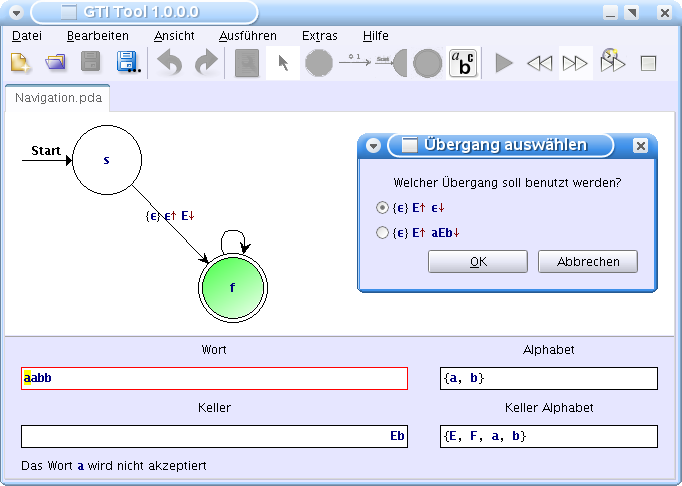
\includegraphics[width=12cm]{../images/grammar_pda.png}
\caption{Operationen mit dem Automaten Keller}
\end{center}
\end{figure}
\vspace{10pt}

Bei dem verwendeten Beispiel kommen zwei Übergänge in Frage. Es könnte der
Übergang gewählt werden, der \Symbol{E} vom Keller liest und nichts auf diesen
schreibt, oder aber der Übergang, der \Symbol{E} vom Keller liest und
\Symbol{a}\Symbol{E}\Symbol{b} auf ihn schreibt. Da \Symbol{a} als nächstes auf
dem Eingabeband steht, sollte der zweite Übergang ausgewählt werden. Dem Benutzer
steht es allerdings frei auch den anderen Übergang auszuwählen. In diesem Fall
würde das Wort \Symbol{a}\Symbol{a}\Symbol{b}\Symbol{b} aber nicht akzeptiert
werden. Der Benutzer hat bei einer falschen Wahl allerdings die Möglichkeit einen
oder mehrere Schritte zurückzugehen, um dann die richtige Wahl zu
treffen.\vspace{10pt}


%%
%% $Id$
%%
%% Copyright (c) 2007-2008 Christian Fehler
%% Copyright (c) 2007-2008 Benjamin Mies
%%


\chapter{Drucken}\label{Print}

Da dieses Lernwerkzeug auch beim Lösen und Nachvollziehen der Übungen
Verwendung finden soll, fanden wir es sehr nützlich und wichtig, dass der
Benutzer seine Lösungen auch ausdrucken kann. Sei es, um diese bei der
Besprechung der Übung zu vergleichen, oder die Ergebnisse auf dem Papier
nochmal nachzuvollziehen.\vspace{10pt}

Daher sind alle Tabellen, welche bei den verschiedenen Funktionen des
Lernwerkzeugs dargestellt werden, druckbar. Weiterhin kann auch der konstruierte
Automat gedruckt werden. Zusätzlich können noch alle Zwischenansichten der
Automaten gedruckt werden, sprich die einzelnen Schritte beim Umwandeln oder
Minimieren.\vspace{10pt}

Desweiteren kann ein konstruierter Automat als Bild exportiert werden. So hat
man die Möglichkeit einen Automaten in ein PDF- oder eine \LaTeX -Datei
einzubinden.\vspace{10pt}


%%
%% $Id$
%%
%% Copyright (c) 2007-2009 Christian Fehler
%% Copyright (c) 2007-2009 Benjamin Mies
%%


%### removes texlipse warnings


\myslide{Konzepte}
{
    \begin{itemgroup}{}
	\item Unterstützung von Lerngruppen
	\item Wenige Eingabebeschränkungen
	\end{itemgroup}

    \vfill{}
}


\myslide{Konzepte - Unterstützung von Lerngruppen}
{
    \begin{itemgroup}{}
	\item Nicht nur Unterstützung einzelner Personen
	\item Unterstützung von Lerngruppen
    \end{itemgroup}

    \begin{itemgroup}{Lösung}
	\item Dateien empfangen
	\item Erstellte Dateien versenden
	\end{itemgroup}
    
    \vfill{}
}


\myslide{Konzepte - Wenige Eingabebeschränkungen}
{
    \begin{itemgroup}{}
	\item Möglichst großer Lernerfolg
	\item Durch Fehler lernen
    \end{itemgroup}

    \begin{itemgroup}{Lösung}
	\item Eingabe so wenig wie möglich einschränken
	\item Einführung von Fehlern und Warnungen
	\item Beispiel: $\epsilon$-Übergang bei einem DEA
	\end{itemgroup}
    
    \vfill{}
}


%### removes texlipse warnings


%%
%% $Id$
%%
%% Copyright (c) 2007-2008 Christian Fehler
%% Copyright (c) 2007-2008 Benjamin Mies
%%


\chapter{Perspektive}\label{Perspective}

In diesem Kapitel werden die Zukunftsperspektiven für das \gtitool besprochen.
Bei der Implementierung wurde besonderer Wert darauf gelegt, dass das \gtitool
leicht zu erweitern sein muss. Der dadurch entstandene Aufwand konnte dadurch
gerechtfertigt werden, dass Erweiterungen in der Zukunft leichter und somit
schneller integriert werden können.\vspace{10pt}


\section{Graphische Komponenten}\label{PerspectiveGraphics}

Wie in Abschnitt \ref{Graph} beschrieben, verwenden wir zur graphischen
Darstellung der Automaten die Bibliothek JGraph. Diese Bibliothek bietet einen
sehr großen Funktionsumfang, der von uns nicht komplett ausgeschöpft werden
musste. Eine mögliche Implementierung für die Zukunft wäre es, diese Bibliothek
durch eine eigene Implementierung zu ersetzen, die dann nur den gewünschten
Umfang bietet und somit leichter zu warten und zu erweitern ist.\vspace{10pt}

Da eine solche Implementierung sehr viel Zeit in Anspruch nehmen würde, war es
uns im Rahmen der Diplomarbeit nicht möglich, neben den umgesetzten Komponenten
auch noch die graphischen Komponenten selbst zu implementieren. JGraph bot uns
die Möglichkeit sehr schnell und einfach bereits brauchbare Ergebnisse zu
erzielen. Es mussten einige in Abschnitt \ref{GraphJGraphAdaptation} beschriebene
Anpassungen vorgenommen werden, damit das Ergebnis unseren Vorstellungen
entsprach, diese waren aber im Gegensatz zu einer vollständigen Implementieren
zeitlich nicht so komplex.\vspace{10pt}

Zu einer möglichen Umsetzung ist zu sagen, dass sowohl Zustände wie auch
Übergänge implementiert werden müssen. Was gerade bei der Verwendung von
parallelen Übergängen ein größeres Problem sein könnte, da dort die Übergänge
nicht auf einer Linie verlaufen. Der größte Nutzer bei einer eigenständigen
Implementierung wäre, dass Änderungen leichter eingepflegt werden könnten, da
dies bei der sehr komplexen Implementierung von JGraph meistens problematisch
war.\vspace{10pt}

Ein weiterer Punkt betrifft die Übergänge. Im Moment verlaufen diese immer
gerade, außer bei parallelen Übergängen. Es wäre aber durchaus wünschenswert,
wenn die Übergänge zum Beispiel um einen Zustand herumgehen würden, wenn dieser
auf dem direkten Weg zwischen zwei Zuständen liegen würde.\vspace{10pt}


\section{Reguläre Ausdrücke}\label{PerspectiveRegEx}

Die wohl wichtigste und komplexeste Erweiterung, die für die Zukunft geplant
ist, ist die Unterstützung von regulären Ausdrücken. Der Benutzer soll somit in
der Lage sein, einen regulären Ausdruck wie
(\Symbol{a}$\mid$\Symbol{b})*\Symbol{a}\Symbol{b}\Symbol{b} eingeben zu können.
Anschließend sollen im Idealfall mehrere Möglichkeiten bestehen, mit diesem
Ausdruck weiter zu arbeiten. Diese Möglichkeiten sollen nun kurz angesprochen
werden.\vspace{10pt}

%### removes texlipse warning
Der eingegebene reguläre Ausdrucks soll mit dem in \cite[S.159ff]{Compilers}
beschriebenen McNaughton-Yamada-Thompson Algorithmus in einen Automaten
umgewandelt werden können. Diese Umwandlung sollte, wie die anderen Umwandlungen
auch, schrittweise durchgeführt werden. Dadurch soll es dem Benutzer ermöglicht
werden, den zur Umwandlung benutzten Algorithmus besser zu verstehen. Abbildung
\ref{FigureThompson} zeigt das Ergebnis, das bei einer solchen Umwandlung
entstehen würde.\vspace{10pt}
%### removes texlipse warning

\begin{figure}[h!]
\begin{center}
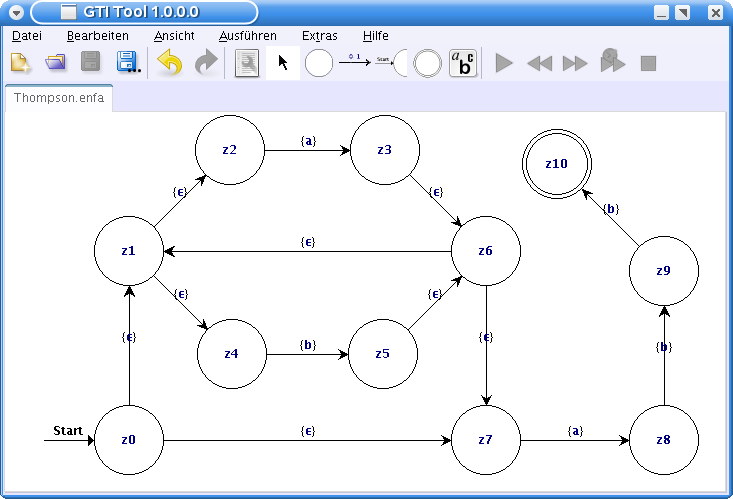
\includegraphics[width=12cm]{../images/thompson.png}
\caption{McNaughton-Yamada-Thompson Algorithmus}
\label{FigureThompson}
\end{center}
\end{figure}
\vspace{10pt}

%### removes texlipse warning
Eine weitere Verwendungsmöglichkeit eines regulären Ausdruck wäre das direkte
Umwandeln in einen DEA. Dieser Algorithmus wird in
\cite[S. 175ff]{Compilers} beschrieben und verwendet die Funktionen
\textit{nullable}, \textit{firstpos}, \textit{lastpos} und \textit{followpos},
um die Umwandlung durchzuführen. Bei der Umsetzung müsste das Berechnen dieser
Funktionen in irgendeiner Weise dargestellt werden, idealerweise anhand des
Syntaxbaumes des regulären Ausdrucks. Ein mögliches Ergebnis der direkten
Umwandlung ist in Abbildung \ref{FigureRegExDFA} zu sehen.\vspace{10pt}
%### removes texlipse warning

\begin{figure}[h!]
\begin{center}
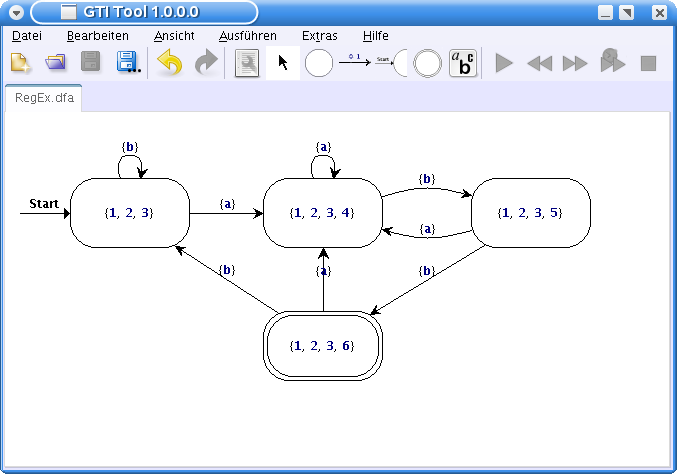
\includegraphics[width=12cm]{../images/regex_dfa.png}
\caption{Direkte Umwandlung in einen DEA}
\label{FigureRegExDFA}
\end{center}
\end{figure}
\vspace{10pt}


\section{\LaTeX-Export}\label{PerspectiveLaTeX}

Bei der Umsetzung des \gtitools war es uns in erster Linie wichtig studentische
Benutzer zu unterstützen. Dazu zählt unter anderem das in Kapitel \ref{Print}
vorgestellte Drucken. Dadurch ist der Benutzer in der Lage, seine erstellten
Automaten oder Grammatiken auszudrucken, um so seine Unterlagen zu
vervollständigen. Eine weitere wichtige Funktion besteht in dem Bildexport.
Durch diesen Export ist der Benutzer in der Lage, die erstellten Automaten als
Bild zu exportieren, um sie zum Beispiel in eigene Prüfungsvorbereitungen
aufzunehmen.\vspace{10pt}

Als Perspektive für die Zukunft wäre es sinnvoll, auch Dozenten besser zu
unterstützen. Eine Möglichkeit wäre das Implementieren eines \LaTeX-Exports, so
dass der Lehrende nicht mehr den Umweg über den Bildexport gehen muss, sondern
den Automaten direkt in \LaTeX\ integrieren kann. Bei der Umsetzung ist auf die
Auswahl einer geeigneten \LaTeX-Bibliothek zu achten, so dass auch große
Automaten noch gut aussehen. Wichtig wäre auch, dass sich, wenn möglich, die
\LaTeX- und die am Bildschirm dargestellte Version wenig
unterscheiden.\vspace{10pt}


\section{Grammatik-Erweiterungen}\label{PerspectiveGrammar}

Bei Grammatiken gibt es noch diverse Möglichkeiten, welche bis jetzt noch nicht
umgesetzt sind. Als Beispiele, auf die wir in diesem Kapitel noch eingehen
möchten, haben wir uns Linksrekursion, Linksfaktorisierung und
Wort-Navigation auf einer Grammatik aufgegriffen.\vspace{10pt}


\subsection{Linksrekursion}\label{PerspectiveLeftrecursion}

Eine Grammatik wird als linksrekursiv bezeichnet, wenn sich aus einem beliebigen
Nichtterminalzeichen $\NonterminalSymbol{A}$ nach beliebig vielen Schritten etwas
von der Form $\NonterminalSymbol{A} \TerminalSymbol{$\alpha$}$ herleiten lässt.
Existiert eine Produktion $\NonterminalSymbol{A} \to \NonterminalSymbol{A}
\TerminalSymbol{$\alpha$}$ spricht man von direkter Linksrekursion. Wenn dazu
mehr als ein Ableitungsschritt nötig ist, spricht man von einer indirekten
Linksrekursion.\vspace{10pt}

%### removes texlipse warning
In \cite{Compilers} ist ein Algorithmus beschrieben, um Linksrekursion
bei einer Grammatik zu beseitigen, welcher sich ohne Probleme umsetzen lassen
sollte.\vspace{10pt}
%### removes texlipse warning

\noindent Gehen wir davon aus, die Produktionen für ein Nichtterminalzeichen
\NonterminalSymbol{A} sind von der Form\vspace{10pt}

\NonterminalSymbol{A} $\to$ \NonterminalSymbol{A}$\alpha_1|\ldots|$
\NonterminalSymbol{A}$\alpha_n | \beta_1 | \ldots | \beta_n$\vspace{10pt}

\noindent wobei $\beta_1\ bis\ \beta_n$ nicht mit \NonterminalSymbol{A}
beginnen.\vspace{10pt}

\noindent Um diese Rekursion zu beseitigen, führt man ein neues
Nichtterminalzeichen \NonterminalSymbol{A$'$} ein. Also ersetzt man die
bestehenden Produktion von
\NonterminalSymbol{A} durch diese Produktionen:\vspace{10pt}

\NonterminalSymbol{A} $\to \beta_1 | \ldots | \beta_n$

\NonterminalSymbol{A$'$} $\to \alpha_1$\NonterminalSymbol{A$'$}$|\ldots|$
$\alpha_n$\NonterminalSymbol{A$'$}$|\epsilon$\vspace{10pt}

%### removes texlipse warning
\noindent Damit können wir direkte Linksrekursion beseitigen. Und dies können wir
uns auch zunutze machen, um indirekte Linksrekursion zu entfernen. Folgender
Algorithmus zur Entfernung von Linksrekursion, aus dem Buch \cite{Compilers},
macht sich dies zu nutze:\vspace{10pt}
%### removes texlipse warning

\noindent
\verb| 1 for i = 1 to n do {|\\
\verb| 2   for j = 1 to i - 1 do {|\\
\verb| 3     ersetze jede Produktion der Form| $A_i \to A_j \gamma$ \verb| |\\ 
\verb| 4     durch die Produktion |$A_i \to \delta_1\gamma|\ldots|\delta_k\gamma$
\verb| 5 , wobei |$A_j \to \delta_1|\ldots|\delta_k$\\ 
\verb| 6     alle derzeitigen Produktionen für |$A_j$ \verb|sind|\\ 
\verb| 7   }|\\
\verb| 8   eleminiere die unmittelbare Linksrekursion für |$A_i$\\
\verb| 9   (mit dem vorhergehend beschriebenen Algorithmus)|\\
\verb|10 }|
\vspace{10pt}

Somit besteht die Möglichkeit sowohl direkte, wie auch indirekte Linksrekursion
zu beseitigen.\vspace{10pt}


\subsection{Linksfaktorisierung}\label{PerspectiveLeftfactorisation}

Bei einer Grammatik kann es zu Problemen kommen, wenn verschiedene Produktionen
gleiche Prefixe haben. Wie es zum Beispiel bei \vspace{10pt}

\noindent
\StartSymbol{S}$ \to$ \TerminalSymbol{if} \NonterminalSymbol{E} \TerminalSymbol{then}
\StartSymbol{S} \TerminalSymbol{else} \StartSymbol{S} $|$ 
\TerminalSymbol{if} \NonterminalSymbol{E} \TerminalSymbol{then} \StartSymbol{S}
\vspace{10pt}

\noindent
der Fall ist. Diese Probleme lassen sich durch den Algorithmus zur
Linksfaktorisierung lösen. Dieser Algorithmus sieht wie folgt aus.\vspace{10pt}

Zunächst einmal bestimmen wir eine Symbolfolge $\alpha$, welche dem längsten
gemeinsamen Prefix aller Produktionen für das selbe Nichtterminalzeichen
\NonterminalSymbol{A} entspricht. In unserem Beispiel wäre $\alpha$ 
"`\TerminalSymbol{if} \NonterminalSymbol{E} \TerminalSymbol{then}
\StartSymbol{S}"'. Alle Produktionen für \NonterminalSymbol{A} sind von der
Form\vspace{10pt}

\noindent
\NonterminalSymbol{A}$ \to \alpha \beta_1|\ldots|\alpha
\beta_n|\gamma_1|\ldots|\gamma_n$
\vspace{10pt}

\noindent
wobei $\gamma$ nicht mit $\alpha$ beginnt und es gilt $n \geq 2$ und $k \geq 0$.
\vspace{10pt}

Um den Algorithmus zur Linksfaktorisierung auf die Grammatik anzuwenden führt
man als erstes ein neus Nichtterminalzeichen \NonterminalSymbol{A$'$} ein. Als
nächstes ersetzt man die bestehenden Produktionen von \NonterminalSymbol{A}
durch die folgenden.\vspace{10pt}

\noindent
\NonterminalSymbol{A}$ \to \alpha $\NonterminalSymbol{A$'$}$|\gamma_1|\ldots|\gamma_n$\\
\NonterminalSymbol{A$'$}$ \to \beta_1|\ldots|\beta_n$
\vspace{10pt}

\noindent
Dieser Schritt muss wiederholt werden, bis für alle Produktionen mit dem
gleichen Nichtterminalzeichen auf der rechten Seite $\epsilon$ der einzige
gemeinsame Prefix ist.\vspace{10pt}

Dieser Algorithmus kann für eine Implementierung verwendet werden, indem für
jedes Nichtterminalzeichen überprüft, ob eine Linksfatorisierung nötig ist, und
diese dann wie oben beschrieben anwendet.


\subsection{Ableitungen für Grammatiken}\label{PerspectiveGrammarWordNavigation}

Die Wortnavigation für Automaten haben wir ja schon in Kapitel
\ref{WordNavigation} beschrieben. Etwas in der Richtung ließe sich
auch für Grammatik realisieren. Allerdings naviert man nicht mehr
durch ein Wort, sondern man sucht die richtig Ableitung von dem
Startsymbol aus.\vspace{10pt}

Dazu könnte die Top-Down Methode des rekursiven Abstiegs verwendet werden. Dieser
Algorithmus startet mit dem Startsymbol der Grammatik auf dem Keller. Wenn
mehrere Produktionen für das Startsymbol in der Grammatik existieren, muss der
Benutzer jetzt auswählen, welches die richtige Produktion ist. Dann wird das
Startsymbol durch die rechte Seite dieser Produktion ersetzt. Jetzt nimmt man
sich jedes Symbol einzeln vor, wobei man von links startet. Handelt es sich um
ein Nichtterminalzeichen, würde dieses wieder durch die rechte Seite der
richtigen nächsten Produktion ersetzt. Handelt es sich um ein Terminalzeichen,
wird dieses mit dem nächsten Zeichen im Eingabewort verglichen. Wenn diese
übereinstimmen wird ein Pointer innerhalb des Eingabewortes ein Symbol
weitergeschoben, und man betrachtet das nächste Symbol. Wenn die beiden Symbole
nicht übereinstimmen, muss eine Fehlermeldung ausgegeben werden, dass dieses Wort
mit den bis jetzt verwendeten Produktionen nich hergeleitet werden kann. Wenn man
das letzte Symbol auf dem Keller behandelt hat, sollte auf dem Keller das
Eingabewort stehen. Somit kann man das Wort mit den Produktionen herleiten, die
man während dieses Durchlaufs verwendet hat. Als Hilfestellung für den Benutzer
sollten diese noch in einer Liste, oder etwas ähnlichem in der Reihenfolge der
Verwendung aufgelistet werden.\vspace{10pt}

\section{Erkannte Wörter ausgeben}\label{PerspectiveDetectedWords}

Eine weitere sinnvolle und für die Zukunft angedachte Erweiterung ist die
Ausgabe von erkannten Wörtern. Nachdem ein Automat, eine Grammatik oder dann
vielleicht auch ein regulärer Ausdruck eingebenen und validiert wurde, soll der
Benutzer in der Lage sein, eine Ansicht zu öffnen, in der er Wörter ausgegeben
bekommt, die zum Beispiel von dem erstellten Automat erkannt
werden.\vspace{10pt}

Bei der Umsetzung ist darauf zu achten, dass die Bestimmung dieser Wörter
möglichst mit geringer Laufzeit implementiert wird, so dass der Benutzer nicht
allzu lange auf ein Ergebnis warten muss. Die Bestimmung sollte somit nicht
einfach per Brute-Force-Methode umgesetzt werden, sondern in irgendeiner Form
abhängig von dem gewendeten Typ sein, wie zum Beispiel einer Grammatik. Somit
sollten gewisse Wörter direkt ausgeschlossen werden, die bei der
Brute-Force-Methode ansonsten mit getestet werden würden.\vspace{10pt}


\section{Eingabe von mehreren Wörtern}\label{PerspectiveMultiplyWordInput}

In der aktuellen Version des \gtitools kann man für Automaten nur ein Wort
eingeben. In Zukunft soll das aber auch für Grammatiken und dann auch für
reguläre Ausdrücke möglich sein. In der aktuellen Umsetzung kann der Benutzer
aber nur ein Wort eingeben und dieses dann auf Akzeptanz prüfen. Für die
Zukunft wäre es somit wünschenswert, mehr als ein Wort eingeben zu können,
welches dann direkt während der Eingabe überprüft wird, so dass der Benutzer
nicht erst die Navigation starten muss. Diese Ansicht soll dem Benutzer helfen, 
zu erkennen, welche Sprache ein erstellter Automat oder eine Grammatik
erkennt.\vspace{10pt}

Eine mögliche Umsetzung wäre, dass Wörter in einer editierbaren Tabelle
eingegeben werden können. Dazu wäre in jeder Zeile ein Parser nötig, der die
Wörter erkennt. Wird eine gültige Eingabe gemacht, kann der Automat dazu
benutzt werden, dieses Wort auf Akzeptanz zu prüfen.\vspace{10pt}


\section{Benutzerinteraktion erhöhen}\label{PerspectiveInteraction}

Bei der Umsetzung des \gtitools war es uns sehr wichtig, dass der Benutzer
bei der Verwendung des Programms möglichst viel lernt. Im Kapitel
\ref{Concepts} wurden einige Konzepte angesprochen, die uns bei der Umsetzung
wichtig erschienen. Aufgrund des vermutlich sehr großen Aufwandes konnten wir
den Bereich Benutzerinteraktion nicht weiter ausbauen. In diesem Abschnitt
werden mögliche Anpassungen angesprochen, die für zukünftige \gtitool Versionen
geplant sind. Bei diesen Anpassungen handelt es sich zum größten Teil um
Erweiterungen der schon implementierten Umsetzungen. Alle in der Zukunft
implementierten Erweiterungen sollten dann direkt mit einer entsprechend hohen
Benutzerinteraktion umgesetzt werden, so dass das nachträgliche Erweitern in
diesen Fällen entfallen würde.\vspace{10pt}


\subsection{Word-Navigation}\label{PerspectiveWordNavigation}
Eine wichtige Erweiterung betrifft die Wort-Navigation. Bei dieser Navigation
gibt es bereits eine Benutzerinteraktion, welche in Abschnitt
\ref{InteractionPDA} beschrieben wird. In Zukunft kann die Benutzerinteraktion,
die in Abschnitt \ref{WordNavigation} beschrieben wird, erweitert werden. Eine
mögliche Umsetzung wäre, den Benutzer vor einem Navigationsschritt dazu
aufzufordern, die Übergänge zu markieren, die als nächstes verwendet werden.
Dabei müsste der Benutzer anhand des nächsten Symbols im Eingabewort entscheiden,
welche Übergänge dies betrifft. Kommen ein oder mehrere $\epsilon$-Übergänge vor,
müssen diese Übergänge zuerst ausgewählt werden. Durch diese Erweiterung würde
der Benutzer noch besser erkennen können, wie der Algorithmus arbeitet. Um den
ungeübten Benutzer nicht zu überfordern und somit vielleicht zur Aufgabe zu
zwingen, muss dieser zusätzliche Auswahlschritt überspringbar sein. Es muss also
eine Art Raten-Funktion geben, die dem Benutzer die Auswahl
abnimmt.\vspace{10pt}


\subsection{Konvertierung}\label{PerspectiveConvertTo}
Im Abschnitt \ref{ConverToMachine} wird das Umwandeln eines Automaten in einen
anderen Automaten beschrieben, also zum Beispiel die Umwandlung von einem
$\epsilon$-NDEA in einen DEA. Der dort implementierte Algorithmus verwendet
verschiedene Phasen. Eine dieser Phasen ist das Bilden des
$\epsilon$-Abschlusses. In diesem Schritt wäre es möglich, den Benutzer alle
Zustände markieren zu lassen, die von dem aktiven Zustand nur durch
$\epsilon$-Übergänge erreichbar sind.\vspace{10pt}

Eine weitere Möglichkeit wäre, den Benutzer dazu aufzufordern, die Zustände zu
aktivieren, die nach einem Übergang mit einem bestimmten Symbol aktiviert sein
werden. Aber auch bei allen anderen Phasen sollte geprüft werden, ob es sinnvoll
wäre, den Benutzer zu einer Interaktion aufzufordern. Es wäre aber nicht nur
möglich, Zustände und Übergänge in dem ursprünglichen Graphen zu markieren,
ebenso wäre es in dem entstehenden Graphen möglich, anzugeben, welche Zustände und
Übergänge in dem nächsten Schritt angelegt werden.\vspace{10pt}


\subsection{Erreichbare Zustände}\label{PerspectiveReachableStates}
Wie im Abschnitt \ref{ReachableStates} vorgestellt, implementiert der
Algorithmus zur Bestimmung der erreichbaren Zustände eine Breitensuche. Bei
dieser Breitensuche könnte der Benutzer dazu aufgefordert werden, die
erreichbaren Zustände zu markieren. Diese Markierung könnte dann überprüft
werden und der Benutzer würde über die Richtigkeit seiner Eingabe informiert.
Auch bei dieser Benutzerinteraktion wäre eine Funktion wichtig, die die
richtige Auswahl trifft.\vspace{10pt}


\subsection{Minimierung}\label{PerspectiveMinimize}
Das Minimieren von Automaten bietet sehr großen Spielraum zum Einbau von
Benutzerinteraktion. Der in Kapitel \ref{Minimize} vorgestellte Algorithmus
basiert darauf, Zustände in Äquivalenz\-klassen zu unterteilen. Es wäre somit
möglich, diese Unterteilung dem Benutzer zu überlassen. Er müsste also
auswählen, warum eine Gruppe in zwei Gruppen zerfällt. Um dies zu erreichen,
müsste der Benutzer Übergänge mit dem gleichen Symbol finden, die in
unterschiedlichen Gruppen enden.\vspace{10pt}

Im ersten Schritt des Minimierens werden die nicht erreichbaren Zustände
entfernt, auch diesen Schritt kann der Benutzer selbst durchführen, in dem er die
entsprechenden Zustände auswählt.\vspace{10pt}


\section{Auto-Layout}\label{PerspectiveAutoLayout}

%###
Wie im Kapitel \ref{AutoLayout} schon erwähnt ist kann der implementierte
Autolayout-Algorithmus noch optimiert werden. Ein Algorithmus welcher
wahrscheinlich bessere Ergebnisse liefert ist der
Simulated-Annealing-Algorithmus (Simulierte Abkühlung), welcher auch in \cite{Layout} beschrieben
wird.\vspace{10pt}
%###

Bei diesem Algorithmus versucht man sich das Verfahren des Abkühlungsprozesses zu
Nutze zu machen, welches in der Natur beobachtet werden kann. Wenn man diesen
Prozess Beispielsweise bei metallischen Schmelzen beobachtet, kann man
feststellen, dass die Metallatome sich zu Beginn des Abkühlunsprozesses noch
annähernd chaotisch durch die Gitterpositionen bewegen. Mit abnehmender
Temperatur nehmen die Atome allerdings immer mehr geordnete Positionen ein, so
dass später nur noch eine Optimierung in der lokalen Nachbarschaft der Atome
möglich ist. Durch dieses Verfahren wird in der Natur immer eine
optimal Lösung erreicht, weshalb man versucht dieses auf ein
Partitionierungsproblem zu übertragen.\vspace{10pt}

Diesen, in der Natur beobachteten Algorithmus, versucht man jetzt nachzubilden,
und mit diesem Verahren Partitionierungsprobleme, beziehungsweise
Layoutprobleme, zu lösen. Dabei gibt man den Elementen zu Beginn einen hohen
Freiheitsgrad, wie es ja auch bei dem Abkühlungsprozess der Fall ist. Dadurch
nimmt man auch Verschlechterungen in Kauf. Dieser Freiheitsgrad nimmt jedoch
immer weiter ab, so dass die Akzeptanz von Verschlechterungen immer weiter
sinkt.\vspace{10pt}

Bei dem Algorithmus werden die Elemente zu Beginn in einer zufällige
Anfangspositionierung gebracht. Jetzt wird über eine Kostenfunktion die
aktuellen Kosten bei dieser Konfiguration berechnet. Als nächstes wählt man
willkürlich zwei Elemente aus und berechnet erneut die Kosten für den Fall,
dass man diese beiden Elemente tauschen würde. Wenn sich die Kosten verbessern
wird der Tausch auf jeden Fall durchgeführt. Wenn die Kosten gleich bleiben,
oder sich sogar verschlechtern würden tauscht man mit einer bestimmten
Wahrscheinlichkeit. Die Maßgebenden Faktoren zur Berechnung der
Wahrscheinlichkeit sind die aktuelle Temperatur und der Grad der
Veschlechterung.\vspace{10pt}

\noindent
Der Pseudocode für diesen Algorithmus sieht wie folgt aus:\vspace{10pt}

\noindent
\verb| 1 begin|\\
\verb| 2   T = T|$_0$\verb|, i = 0|\\
\verb| 3   cur_part = init_part|\\
\verb| 4   cur_cost=COST( cur_part )|\\
\verb| 5   repeat|\\
\verb| 6     repeat|\\
\verb| 7       i = i + 1|\\
\verb| 8       a|$_i$\verb| = SELECT( A ), b|$_i$\verb| = SELECT( B )|\\
\verb| 9       trial_part = EXCHANGE( a|$_i$\verb|,b|$_i$\verb|, cur_part )|\\
\verb|10       trial_cost = COST( trial_part )|\\
\verb|11       |$\Delta$\verb|cost = trial_cost - cur_cost|\\
\verb|12       if ( |$\Delta$\verb|cost < 0 ) then|\\
\verb|13         cur_cost = trial_cost|\\
\verb|14         cur_part = MOVE ( a|$_i$\verb|, b|$_i$\verb| )|\\
\verb|15       else|\\
\verb|16         r = RANDOM ( 0, 1 )|\\
\verb|17         if ( r < e|$^{-\frac{\Delta cost}{T}}$\verb| ) then|\\
\verb|18           cur_cost = trial_cost|\\
\verb|19           cur_part = MOVE ( a|$_i$\verb|, b|$_i$\verb| )|\\
\verb|20     until (Abbruchskriterium, z.B. Gleichgewicht bei T, erreicht)|\\
\verb|21    T = |$\alpha$\verb| * T|\\
\verb|22   until ( T < T|$_{min}$\verb| )|\\
\verb|23 end|\\ 
\vspace{10pt}

Die Kostenfunktion ist bei der Implementierung des Algorithmus ein wichtiger
Punkt aus. In unserem speziellen Fall müsste man berücksichtigen, dass zwei
Zustände, zwischen denen ein Übergang existiert, nicht zu weit auseinanderliegen
sollten. Wenn zwei Zustände nicht direkt nebeneinander liegen können, sollte sehr
großer Wert darauf gelegt werden, dass der Übergang nicht durch einen anderen
Zustand geht, so dass die Beschriftung des Übergangs oder des anderen Zustandes
eventuell nicht mehr zu erkennen ist. Weiterhin sollten die Überschneidungen der
Übergänge untereinander möglichst gering sein.
\vspace{10pt}


\setcounter{secnumdepth}{-1}
%%
%% $Id$
%%
%% Copyright (c) 2007-2009 Christian Fehler
%% Copyright (c) 2007-2009 Benjamin Mies
%%


%### removes texlipse warnings


\chapter{Fazit}\label{Conclusion}

Das von uns implementierte \gtitool wurde entwickelt, um den Benutzern die
Grundlagen der theoretischen Informatik näher zu bringen. Ob dies gelungen ist,
wird der Einsatz der Software in der Zukunft zeigen. Um dieses Ziel zu erreichen,
wurden alle einzelnen Komponenten des Programms zusammen geplant und anschließend
eng verzahnt von uns beiden umgesetzt. Bei dieser Umsetzung war immer einer
hauptverantwortlich für den jeweiligen Bereich. Je nach Erfahrung ergänzten wir
uns allerdings bei der Umsetzung, um möglichst effizient arbeiten zu
können.\vspace{10pt}

Bei der Implementierung war es uns wichtig in etwa den gleichen Umfang des
Programms Machines (siehe \cite{machines}) zu erreichen oder so vorzubereiten,
dass er in Zukunft erreicht werden kann. Eine eigene Implementierung war
wichtig, da Machines nicht ganz zu der Vorlesung passte und in einigen Punkten
aus unserer Sicht verbesserungswürdig erschien. So werden Algorithmen zu wenig
detailreich umgesetzt und die Bedienung ist zum Teil wenig intuitiv. Aus diesen
Gründen war eine eigenständige Implementierung, die an die aktuelle Vorlesung
angepasst werden kann, sehr hilfreich.\vspace{10pt}

Bei der ersten Planung bzw. Vorbesprechung der Diplomarbeit wurden die Ziele in
den Vordergrund gestellt, verschiedene Automaten und Grammatiken zu
unterstützen. Während der Implemtierung wurden immer genauere Ziele gesteckt
bzw. bestehende Ziele eingegrenzt. So entstand die Umwandlung der Automaten in
andere Automaten oder die Umwandlung von Grammatiken in Automaten. Ein weiteres
Beispiel für die nachträgliche Anpassung der Ziele ist die Umsetzung der
erreichbaren Zustände. Die Notwendigkeit eines solchen Algorithmus entstand
durch das Umwandeln unter Verwendung eines Potenzautomaten. Da bei einer
solchen Umwandlung sehr große Automaten entstehen können, wurde das im
Abschnitt \ref{ReachableStates} vorgestellte Verfahren notwendig.\vspace{10pt}

Bei der Umsetzung des \gtitools war es uns sehr wichtig, dass wir eine
qualitativ hochwertige Software entwickeln. Dies betrifft sowohl das
Aussehen des Programms, aber auch den Source Code. Durch diese angestrebte hohe
Qualität wurde in Kauf genommen, dass quantitativ nicht alle Komponenten
umgesetzt werden konnten.\vspace{10pt}

Im Kapitel \ref{Perspective} wurden einige Perspektiven für die Zukunft
vorgestellt, da wir davon ausgehen, dass unsere Software in Zukunft
weiterentwickelt wird, um dem Benutzer eine noch bessere Unterstützung zur
Verfügung zu stellen. Der Nachteil quantitativ weniger erreicht zu haben wurde
damit gerechtfertigt, dass die Software leichter zu erweitern ist, wodurch
zukünftige Erweiterungen schneller und weniger fehleranfällig integriert werden
können. Ein weiterer Vorteil dieser Umsetzung ist, dass in Zukunft auftauchende
Fehler leichter und somit schneller beseitigt werden können.\vspace{10pt}

Abschließend bleibt zu sagen, dass die Planung und die anschließende
Implementierung des \gtitools sehr viel Freude gemacht hat. Wir hoffen, dass sich
der Aufwand gelohnt hat und, dass wir den Studenten die theoretischen Inhalte der
Informatik näher gebracht haben. Gleichfalls würden wir uns freuen, wenn unsere
Software in Zukunft weiterentwickelt würde, um weitere Funktionen zu
ergänzen.\vspace{10pt}


%### removes texlipse warnings

\setcounter{secnumdepth}{2}

\bibliographystyle{alphadin}
\bibliography{literature}

\setcounter{secnumdepth}{-1}
%%
%% $Id$
%%
%% Copyright (c) 2007-2008 Christian Fehler
%% Copyright (c) 2007-2008 Benjamin Mies
%%


%### removes texlipse warnings


\chapter{Aufteilung}\label{Partition}

Im folgenden eine Übersicht, die Auskunft darüber gibt, wer von uns welchen
Teil dieser Diplomarbeit geschrieben hat.


\begin{longtable}{|p{1.30cm}@{}p{7.55cm}@{}p{3.00cm}@{}|}
  \hline

  &
  \textbf{Einleitung}&
  \bm\\
  
  \hline

  \ref{GUI}&
  \textbf{Oberfläche}&
  \cf\\
  \ref{GUIMain}&
  Gestaltung der Hauptansicht&
  \bm\\
  \ref{GUIDesign}&
  Gestaltung der graphischen Komponenten&
  \bm\\
  \ref{GUIRedoUndo}&
  Redo/Undo&
  \bm\\
  \ref{GUIAdaption}&
  Anpassung aller GUI Komponenten&
  \cf\\
  \ref{LookAndFeel}&
  Look \& Feel&
  \cf\\
  \ref{SecondView}&
  Zweite Ansicht&
  \cf\\
  \ref{Parser}&
  Parser&
  \cf\\
  \ref{ParserContext}&
  Kontextsensitive Bedingungen&
  \cf\\
  \ref{ParserAdaption}&
  Anpassung der Darstellungsweise&
  \cf\\
  \ref{Print}&
  Drucken&
  \bm\\
  
  \hline

  \ref{Machines}&
  \textbf{Automaten}&
  \cf\\
  \ref{Graph}&
  Graphenansicht&
  \cf\\
  \ref{GraphJGraph}&
  Automatendarstellung mit JGraph&
  \bm\\
  \ref{GraphJGraphAdaptation}&
  Anpassung von JGraph&
  \cf\\
  \ref{Tables}&
  Tabellen&
  \cf\\
  \ref{TablesTransition}&
  Übergangstabelle&
  \cf\\
  \ref{TablesPDA}&
  Tabelle für Keller-Operationen&
  \bm\\
  \ref{WordNavigation}&
  Wort-Navigation&
  \cf\\
  \ref{WordNavigationDeterministic}&
  Deterministische Navigation&
  \bm\\
  \ref{HistoryPath}&
  Zustands Pfad&
  \cf\\
  \ref{InteractionPDA}&
  Operationen mit dem Automaten Keller&
  \cf\\
  \ref{ReachableStates}&
  Erreichbare Zustände&
  \cf\\
  \ref{ConverToMachine}&
  Konvertierung&
  \cf\\
  \ref{Minimize}&
  Minimierung&
  \bm\\
  \ref{AutoLayout}&
  Auto Layout&
  \bm\\
  \ref{KerninghanLin}&
  Der Kerninghan-Lin-Algorithmus&
  \bm\\
  \ref{InteractionMachine}&
  Fehler und Warnungen&
  \cf\\
  
  \hline
\end{longtable}

\newpage

\begin{longtable}{|p{1.30cm}@{}p{7.55cm}@{}p{3.00cm}@{}|}
  \hline

  \ref{Grammars}&
  \textbf{Kontextfreie Grammatiken}&
  \bm\\
  \ref{ConverToGrammar}&
  Grammatik Konvertierung&
  \bm\\
  \ref{ConverToGrammarRegular}&
  Konvertierung einer regulären Grammatik&
  \bm\\
  \ref{ConverToGrammarContextFree}&
  Konvertierung einer kontextfreien Grammatik&
  \bm\\
  \ref{InteractionGrammar}&
  Fehler und Warnungen&
  \bm\\

  \hline

  \ref{Perspective}&
  \textbf{Perspektiven}&
  \cf\\
  \ref{PerspectiveGraphics}&
  Graphische Komponenten&
  \cf\\
  \ref{PerspectiveRegEx}&
  Reguläre Ausdrücke&
  \cf\\
  \ref{PerspectiveLaTeX}&
  \LaTeX-Export&
  \cf\\
  \ref{PerspectiveGrammar}&
  Grammatik Erweiterungen&
  \bm\\
  \ref{PerspectiveLeftrecursion}&
  Linksrekursion&
  \bm\\
  \ref{PerspectiveLeftfactorisation}&
  Linksfaktorisierung&
  \bm\\
  \ref{PerspectiveGrammarWordNavigation}&
  Wortnavigation für Grammatiken&
  \bm\\
  \ref{PerspectiveDetectedWords}&
  Erkannte Wörter ausgeben&
  \cf\\
  \ref{PerspectiveMultiplyWordInput}&
  Eingabe von mehreren Wörtern&
  \cf\\
  \ref{PerspectiveInteraction}&
  Benutzerinteraktion erhöhen&
  \cf\\
  \ref{PerspectiveWordNavigation}&
  Wort-Navigation&
  \cf\\
  \ref{PerspectiveConvertTo}&
  Konvertierung&
  \cf\\
  \ref{PerspectiveReachableStates}&
  Erreichbare Zustände&
  \cf\\
  \ref{PerspectiveMinimize}&
  Minimierung&
  \cf\\
  \ref{PerspectiveAutoLayout}&
  Auto-Layout&
  \bm\\
  
  \hline

  &
  \textbf{Fazit}&
  \cf\\

  \hline
\end{longtable}


%### removes texlipse warnings

\setcounter{secnumdepth}{2}

\setcounter{secnumdepth}{-1}
%%
%% $Id$
%%
%% Copyright (c) 2007-2009 Christian Fehler
%% Copyright (c) 2007-2009 Benjamin Mies
%%


%### removes texlipse warnings


\chapter{Erklärung}

\thispagestyle{empty}

Hiermit versichere ich, dass ich die im Abschnitt Aufteilung angegebenen Teile
der vorliegende Diplomarbeit selbstst\"andig verfasst habe und keine anderen als
die angegebenen Hilfsmittel und Quellen benutzt habe.\vskip 1cm
\begin{tabular}{lc}
Siegen, den \date{\ClosingDate} & \rule{6.5cm}{0.5pt} \\
                   & (Christian Fehler)
\end{tabular}\vskip 2cm

\noindent
Hiermit versichere ich, dass ich die im Abschnitt Aufteilung angegebenen Teile
der vorliegende Diplomarbeit selbstst\"andig verfasst habe und keine anderen als
die angegebenen Hilfsmittel und Quellen benutzt habe.\vskip 1cm
\begin{tabular}{lc}
Siegen, den \date{\ClosingDate} & \rule{6.5cm}{0.5pt} \\
                   & (Benjamin Mies)
\end{tabular}


%### removes texlipse warnings

\setcounter{secnumdepth}{2}

\setcounter{secnumdepth}{-1}
\chapter{Anhang}
\setcounter{secnumdepth}{2}

\end{document}